\documentclass[preprint,authoryear,number]{elsarticle}
\usepackage{setspace}
\setlength{\parskip}{0.5em}
\setlength{\footnotesep}{12pt}

\usepackage[utf8]{inputenc}
\usepackage[T1]{fontenc}
\usepackage{amsmath,amssymb}
\usepackage{graphicx}
\usepackage{booktabs}
\usepackage{multirow}
\usepackage{xcolor}
\usepackage{hyperref}
\usepackage{siunitx}
\usepackage{lineno}
\usepackage{natbib}

\modulolinenumbers[5]
\linenumbers

\journal{Earth Science Informatics}

\begin{document}

\begin{frontmatter}

\title{Symbolic Regression for Automated Spectral Feature Engineering: A Leakage-Free Framework Evaluated on Sentinel-2 Alteration Mapping}

\author[usach]{Francisco Parra~O.\corref{cor1}}
\ead{francisco.parra.o@usach.cl}
\cortext[cor1]{Corresponding author}

\author[dim]{Gonzalo R\'ios}

\author[uoh,systemix,cgr,cmm,inta]{Mauricio Latorre}

\address[usach]{Universidad de Santiago de Chile (USACH), Santiago, Chile}
\address[dim]{Departamento de Ingenier\'ia Matem\'atica, Facultad de Ciencias F\'isicas y Matem\'aticas, Universidad de Chile, Santiago, Chile}
\address[uoh]{Laboratorio de Bioingenier\'ia, Instituto de Ciencias de la Ingenier\'ia, Universidad de O'Higgins, Libertador Bernardo O'Higgins 611, Rancagua, Chile}
\address[systemix]{Centro de Biolog\'ia de Sistemas para el Estudio de Comunidades Extrem\'ofilas de Relaves Mineros (SYSTEMIX), Universidad de O'Higgins, Libertador Bernardo O'Higgins 611, Rancagua, Chile}
\address[cgr]{Millennium Institute Center for Genome Regulation, Santiago 8320165, Regi\'on Metropolitana, Chile}
\address[cmm]{Center for Mathematical Modeling, University of Chile, Beauchef 851, Santiago, Chile}
\address[inta]{Laboratorio de Bioinform\'atica y Expresi\'on G\'enica, INTA, Universidad de Chile, El L\'ibano 5524, Macul, Santiago, Chile}

\begin{abstract}
We present symbolic regression (SR) as a general-purpose framework for automated and interpretable spectral feature engineering in multispectral classification. The framework requires only labeled pixels and a sensor's band configuration as input, and can be re-applied at any new site to discover locally optimal formulas. Because SR discovery is label-dependent, the complete pipeline (formula discovery $\rightarrow$ feature transformation $\rightarrow$ classification) is evaluated under nested cross-validation, in which PySR is re-run exclusively on the training partition of each outer fold. Discovery is therefore never exposed to test pixels. We demonstrate the approach on hydrothermal alteration mapping with Sentinel-2, a challenging test case with six spectrally similar classes. Training used field-mapped ground truth from Chile's Atacama Region, with two geologically independent validation sites: Chile's Coquimbo Region (\SI{200}{\kilo\meter} distant, same metallogenic belt) and Cuprite, Nevada, USA (different continent and geological province). Two findings emerge. First, SR-derived and classical indices are complementary. A Random Forest on six SR features plus seven classical indices significantly outperforms the same classifier on all ten raw Sentinel-2 bands, under both stratified nested cross-validation (mean AUC 0.917 vs.\ 0.899, $p = 0.002$) and polygon-disjoint spatial nested cross-validation, which removes autocorrelation between adjacent pixels (0.838 vs.\ 0.822, $p = 0.008$). It does so with fewer features than the raw-plus-classical alternative. Second, the six SR features alone retain 98--99\% of the discriminative performance of the ten raw bands (nested mean AUC 0.889 vs.\ 0.899; 0.802 vs.\ 0.822 under spatial validation). This quantifies an honest discovery cost of 0.01--0.02 AUC that in-sample evaluation designs underestimate. Discovery is also stable across folds. The strongest formulas, including the propylitic index $B_{03} - 0.48 \cdot B_{11}$ (standalone AUC = 0.91 on a locked hold-out, DeLong $p < 0.001$ against classical indices), are rediscovered nearly verbatim in independent training partitions. Both findings replicate at Cuprite with locally discovered formulas (SR $+$ classical 0.939 vs.\ raw 0.933; SR alone 0.920), and a cross-domain proof-of-concept on land cover classification (SR $+$ classical AUC 0.926 vs.\ raw 0.920) supports generalization beyond geological applications. Physical interpretation confirms that discovered formulas exploit mineral absorption mechanisms consistent with spectroscopic theory. The methodology is sensor-agnostic, reproducible, and applicable to a broad range of multispectral classification problems where labeled pixels are available and compact, auditable features are preferred over black-box models.
\end{abstract}

\begin{keyword}
symbolic regression \sep spectral indices \sep automated feature engineering \sep multispectral classification \sep Sentinel-2 \sep hydrothermal alteration \sep interpretable machine learning
\end{keyword}

\end{frontmatter}

%% Highlights (submitted as separate file)
%% - Leakage-free nested CV: symbolic regression re-run inside every training fold
%% - SR + classical features significantly beat all raw bands (AUC 0.917 vs 0.899)
%% - Six SR features alone retain 98-99% of the raw-band discriminative performance
%% - Complementarity replicates across continents with locally discovered formulas
%% - Propylitic SR index significantly outperforms classical indices (DeLong p<0.001)

%% ============================================================
\section{Introduction}
\label{sec:introduction}

Remote sensing of hydrothermal alteration minerals is fundamental to geological exploration and geothermal resource assessment \citep{Sabins1999,vanderMeer2012,Pour2018}. The spectral signatures of alteration minerals (particularly absorption features related to OH-bearing phases, iron oxides, and silicates)enable their detection from multispectral and hyperspectral satellite imagery \citep{Hunt1977,Clark1999}. Over the past three decades, spectral indices such as band ratios and normalized differences have been the primary tools for mapping alteration zones from satellite data \citep{Ninomiya2005,Mars2010}.

The majority of established hydrothermal alteration indices were designed for the Advanced Spaceborne Thermal Emission and Reflection Radiometer (ASTER), which provides five shortwave infrared (SWIR) bands between \SIrange{1.6}{2.43}{\micro\meter} at \SI{30}{\meter} resolution \citep{Ninomiya2005,Mars2006}. These include the Kaolinite Index (KLI), Alunite Index (ALI), and OH-bearing minerals Index (OHI), all of which exploit subtle absorption differences within the SWIR region \citep{Ninomiya2005}. However, ASTER's limited temporal coverage (on-demand acquisition) and the aging of its SWIR subsystem have motivated the adoption of alternative sensors for geological applications.

Sentinel-2, operated by the European Space Agency's Copernicus programme, offers global coverage at \SIrange{10}{20}{\meter} resolution with a 5-day revisit period \citep{Drusch2012}. While Sentinel-2 has only two SWIR bands (B11 at \SI{1610}{\nano\meter} and B12 at \SI{2190}{\nano\meter}) compared to ASTER's five, it compensates with higher spatial resolution, more frequent acquisitions, four red edge bands (\SIrange{705}{865}{\nano\meter}), and free global access. Several studies have adapted ASTER-derived ratios to Sentinel-2 \citep{vanderWerff2016,Ge2018,Shirmard2022}, but these adaptations do not exploit the full spectral potential of the sensor's 13-band configuration.

The design of spectral indices has traditionally relied on expert knowledge of mineral spectroscopy \citep{Hunt1977,Clark1999}. While effective, this approach is inherently limited to the hypotheses that domain experts formulate. An alternative is to let the data determine optimal spectral formulas through automated search. Symbolic regression (SR) is a machine learning technique that searches the space of mathematical expressions to find compact, interpretable formulas that fit the data \citep{Koza1992,Cranmer2023}. Unlike neural networks or ensemble methods, SR produces closed-form expressions that can be directly interpreted, reproduced, and applied in any geographic information system (GIS) environment. Recent advances in SR algorithms, particularly the PySR library \citep{Cranmer2023}, have made large-scale symbolic search computationally tractable.

To our knowledge, no prior study has applied symbolic regression to discover spectral indices for hydrothermal alteration mapping. The closest related work involves automated spectral feature selection for lithological mapping \citep{Shirmard2022} and curated databases of spectral indices such as the Index Database \citep{Henrich2012}. Deep learning approaches have achieved high accuracy in alteration mapping \citep{Shirmard2022,Ye2017}, but their black-box nature limits physical interpretability and practical adoption by the geological community.

In this study, we address the following research questions: \emph{(1) Can symbolic regression automatically discover compact, interpretable spectral formulas that match the discriminative power of raw multispectral bands? (2) Does this automated feature engineering framework generalize across geological provinces and continents?} We emphasize the distinction between \emph{formula transferability} (whether a specific discovered formula works at a new site) and \emph{method transferability} (whether the SR-based discovery process produces equally effective features at a new site). The latter is the primary contribution: we show that the framework (not any particular formula)is the transferable product. We demonstrate the methodology on hydrothermal alteration mapping with Sentinel-2 (a domain where expert-designed indices have dominated for three decades)as a challenging test case with six spectrally similar target classes, validated at three sites spanning two continents and two distinct geological provinces.

Our contributions are fourfold.
\begin{enumerate}
  \item We introduce a general, re-deployable symbolic regression framework for automated spectral feature engineering from multispectral imagery, together with a leakage-free evaluation protocol for it: because formula discovery is label-dependent, the complete pipeline (discovery $\rightarrow$ transformation $\rightarrow$ classification) is evaluated under nested cross-validation, with PySR re-run exclusively inside each outer training fold.
  \item We show that SR-derived and classical indices capture complementary information: their combination significantly outperforms the ten raw Sentinel-2 bands under both stratified nested CV (mean AUC 0.917 vs.\ 0.899, $p = 0.002$) and polygon-disjoint spatial nested CV (0.838 vs.\ 0.822, $p = 0.008$), and does so with fewer features than augmenting the raw bands with the same classical indices. This pattern is confirmed across four classifiers and two deep learning architectures.
  \item We quantify the honest cost of automated discovery: six SR features alone retain 98--99\% of the raw-band discriminative performance (nested AUC 0.889 vs.\ 0.899 stratified; 0.802 vs.\ 0.822 polygon-disjoint), a 0.01--0.02 AUC discovery cost that in-sample evaluation designs underestimate. Unlike PCA-based reduction, which achieves higher absolute AUC through opaque linear combinations, each SR feature is a closed-form expression with a direct mineral-spectroscopic interpretation, deployable in any raster calculator without a fitted transformation.
  \item We demonstrate that both findings replicate at a geologically independent benchmark in Cuprite, Nevada (USA), using formulas discovered locally by the identical configuration, confirming that what transfers across continents and geological provinces is the discovery framework, not any particular formula.
\end{enumerate}


%% ============================================================
\section{Study Areas}
\label{sec:study_areas}

\subsection{Training Site: Atacama Region (III), Chile}

The primary study area encompasses the metallogenic belt of Chile's Atacama Region (III), centered on the Maricunga district (\ang{-26.85} S, \ang{-69.2} W; Fig.~\ref{fig:study_area}a,b). This area hosts extensive hydrothermal alteration associated with Tertiary (Oligocene--Miocene) volcanic and porphyry copper--gold systems within the Central Andes \citep{Sillitoe1991,Vila1991}. Host lithologies include andesitic to dacitic volcanic sequences, subvolcanic porphyry intrusions, and associated volcaniclastic sediments at elevations of \SIrange{3500}{5000}{\meter}. The geological mapping of alteration zones has been systematically documented in the \emph{Atlas Metal\'ifero de la III Regi\'on} published by Chile's Servicio Nacional de Geolog\'ia y Miner\'ia (SERNAGEOMIN), which includes field-mapped polygons classified by alteration type.

The mapped alteration types include: (1)~silicic alteration (vuggy silica, quartz--alunite cores), (2)~advanced argillic alteration (kaolinite, alunite, pyrophyllite), (3)~argillic and phyllic alteration (illite, sericite, montmorillonite), (4)~propylitic alteration (chlorite, epidote, calcite), (5)~iron oxide zones (goethite, hematite, jarosite), and (6)~potassic alteration and skarn (biotite, K-feldspar, calc-silicate minerals). The atlas contains 92 classified alteration polygons and 544 polygons labeled as ``undifferentiated hydrothermal alteration.''

The arid climate of the Atacama Desert (\textless\SI{50}{\milli\meter} annual precipitation) provides near-ideal conditions for spectral remote sensing, with minimal vegetation cover and atmospheric moisture effects.

\subsection{Validation Site: Coquimbo Region (IV), Chile}

The cross-site validation area is located in Chile's Coquimbo Region (IV), approximately \SI{200}{\kilo\meter} south of the training site. This region shares the same Andean metallogenic context but with different host lithologies and alteration geometries, providing a geologically independent test of formula generalization within the same metallogenic province. Alteration mapping from SERNAGEOMIN geological surveys provides ground truth for four classes: silicic, advanced argillic, argillic-phyllic, and propylitic.

\subsection{External Validation Site: Cuprite, Nevada, USA}

To test whether the SR feature engineering approach generalizes beyond the Chilean Andes, we selected the Cuprite mining district (\ang{37.5} N, \ang{-117.2} W) in Esmeralda County, Nevada, USA. Cuprite is the most widely used benchmark site for spectral remote sensing of hydrothermal alteration \citep{Swayze2014} and represents a fundamentally different geological context: late Miocene advanced argillic alteration in a Basin and Range extensional setting, versus Tertiary porphyry-related alteration in the Andean compressional belt.

Ground truth was derived from the USGS digital map of hydrothermal alteration for the southwestern United States \citep{Rockwell2017}, accessed via the USGS Web Map Service (WMS) at \texttt{mrdata.usgs.gov/services/alteration}. The alteration raster, produced by automated analysis of ASTER imagery using the Tetracorder system, provides four classes compatible with our framework: silicic (hydrothermal silica), argillic, phyllic (muscovite/illite), and propylitic (epidote/chlorite and carbonate). A total of 20{,}000 Sentinel-2 pixels were sampled within the Cuprite area, of which 3{,}466 (17.3\%) fell within USGS-mapped alteration zones: 1{,}831 silicic, 581 argillic, 514 phyllic, and 540 propylitic. The USGS ``argillic'' class corresponds to our advanced argillic (kaolinite/alunite-dominated), while ``phyllic'' maps to our argillic-phyllic (muscovite/illite). The USGS propylitic class (epidote/chlorite + carbonate) matches our propylitic definition. Iron oxide and potassic-skarn classes are not distinguished in the USGS alteration product.

\begin{figure*}[ht]
\centering
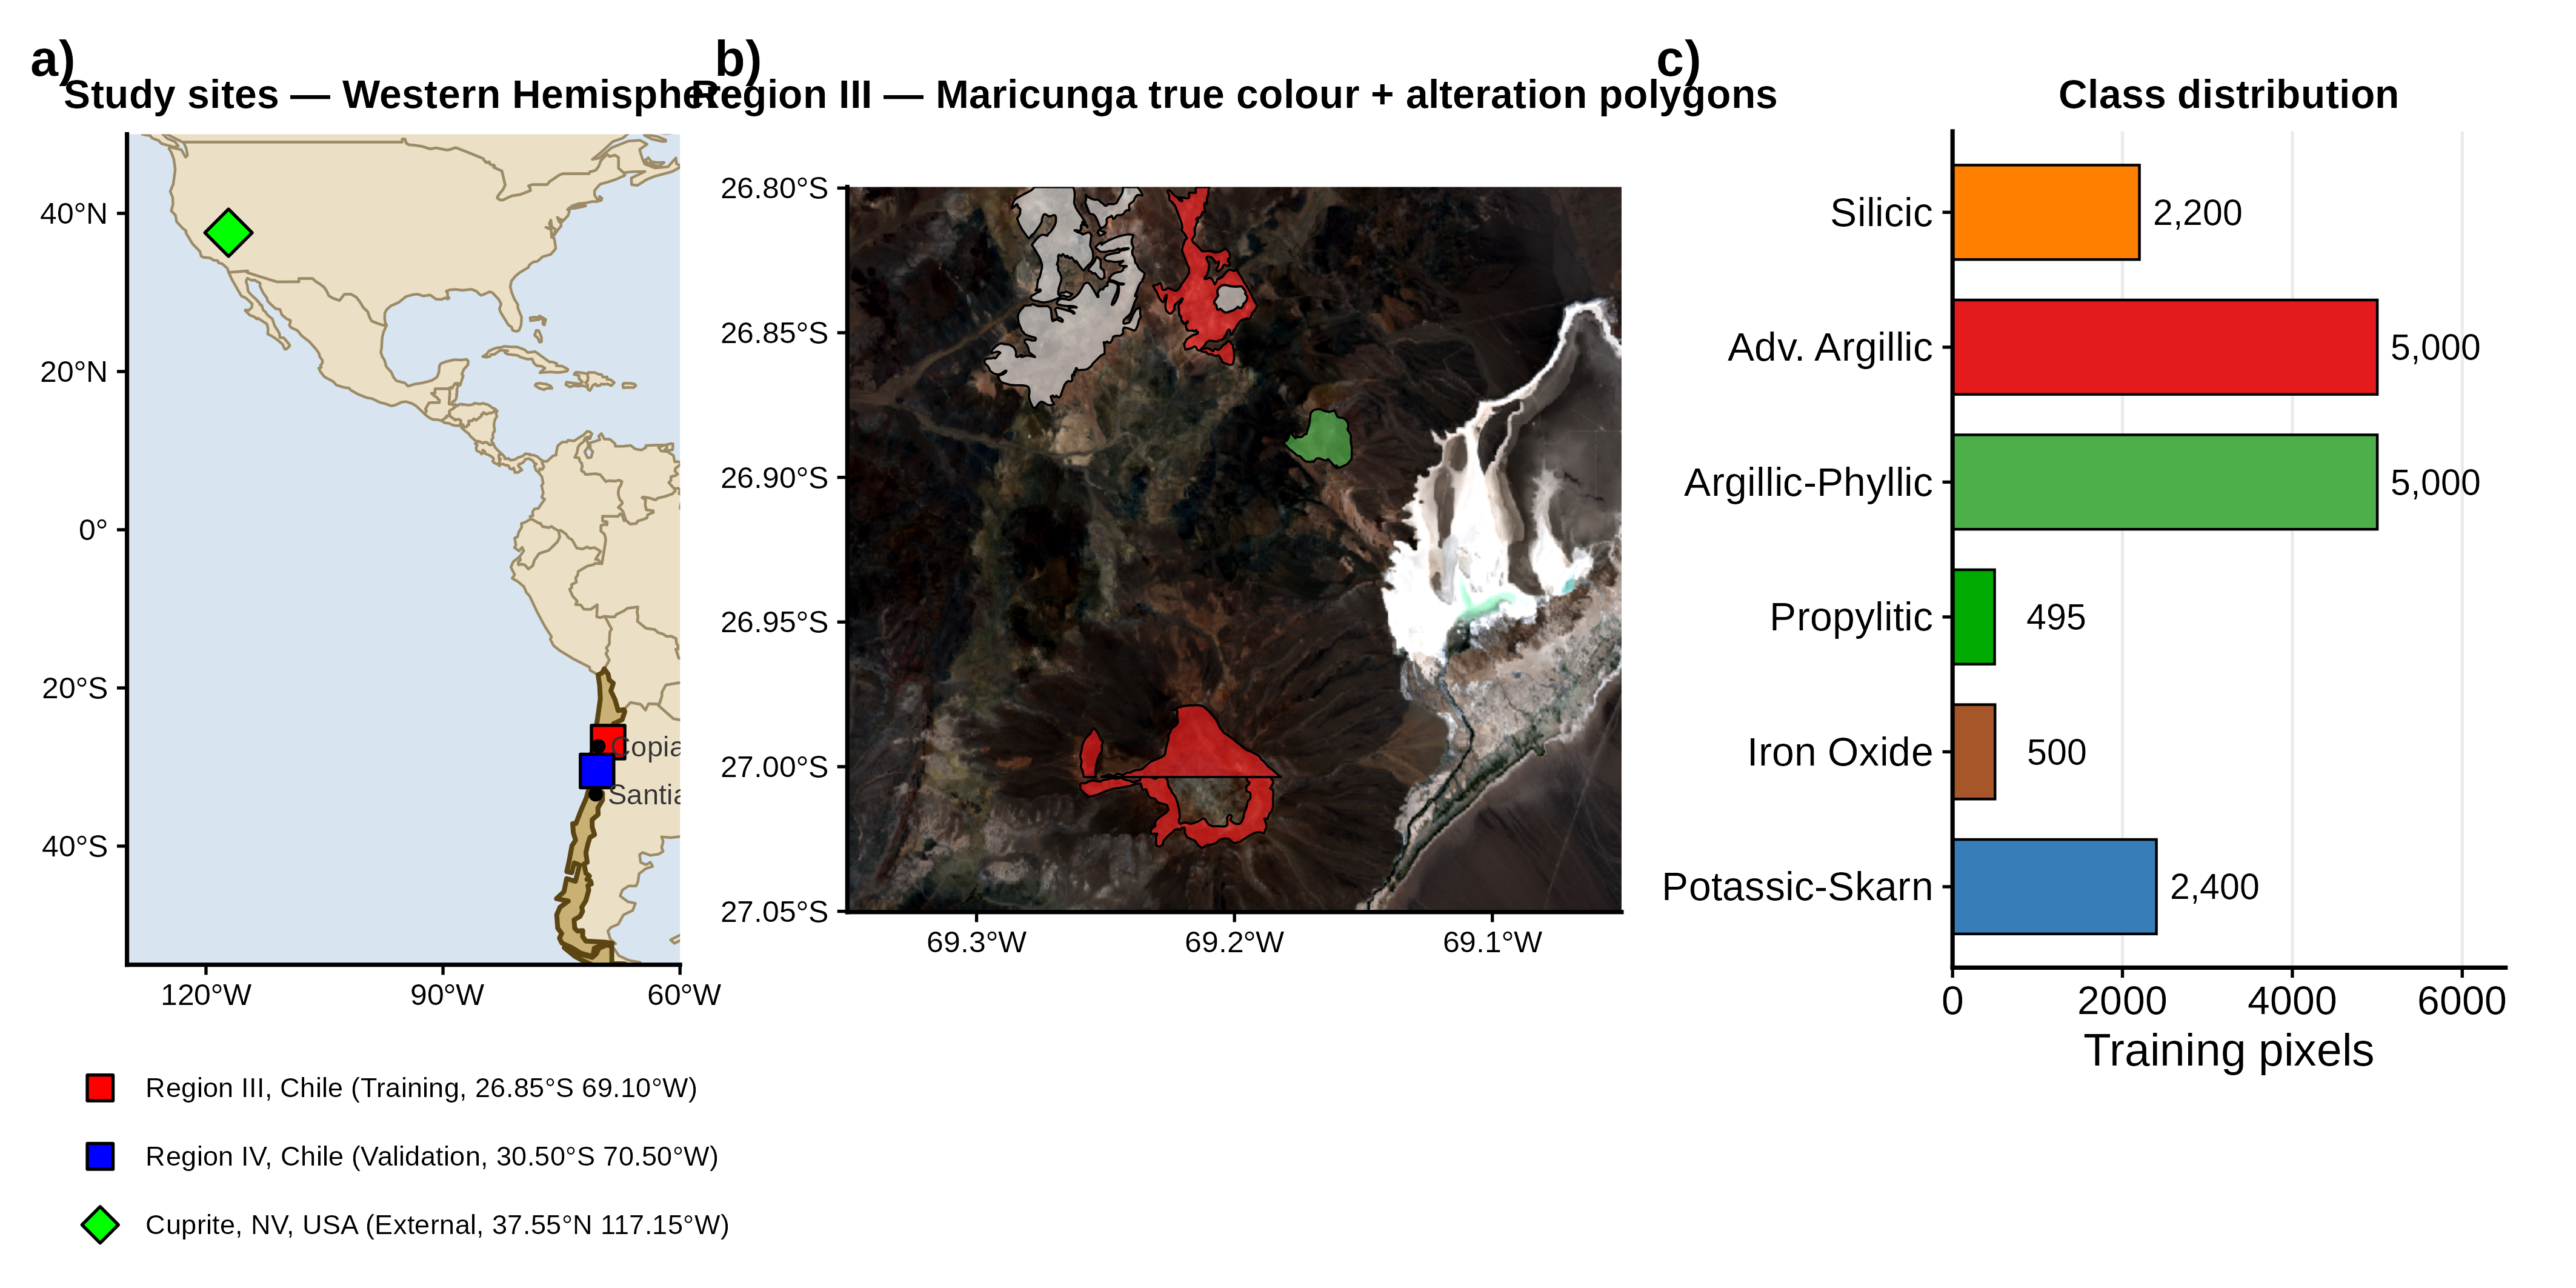
\includegraphics[width=\textwidth]{../figures/study_area.png}
\caption{Study areas and ground truth data. (a)~Location in Chile showing the training site (Region~III, red) and validation site (Region~IV, blue). Dashed box indicates Sentinel-2 coverage. (b)~Alteration polygons from the Atlas Metal\'ifero de la III Regi\'on, color-coded by alteration type. Gray polygons represent undifferentiated hydrothermal alteration. (c)~Distribution of training pixels across alteration classes. The external validation site at Cuprite, Nevada (\ang{37.5} N, \ang{-117.2} W) is not shown; ground truth was derived from the USGS ASTER-based alteration map \citep{Rockwell2017}. Map lines delineate study areas and do not necessarily depict accepted national boundaries.}
\label{fig:study_area}
\end{figure*}


%% ============================================================
\section{Data and Methods}
\label{sec:methods}

\subsection{Sentinel-2 Data Acquisition and Preprocessing}

We used Sentinel-2 Level-2A (L2A) surface reflectance imagery from the Copernicus/S2\_SR\_HARMONIZED collection accessed through Google Earth Engine \citep{Gorelick2017}. For the Chilean sites, we selected scenes from the dry season (January--March 2024) with cloud cover below 20\%. For Cuprite, Nevada, scenes from the summer dry season (June--September 2024) were used with the same cloud threshold. A temporal median composite was computed to reduce atmospheric residuals and noise.

Ten spectral bands were retained for analysis (Table~\ref{tab:s2bands}): B02 (Blue, \SI{490}{\nano\meter}), B03 (Green, \SI{560}{\nano\meter}), B04 (Red, \SI{665}{\nano\meter}), B05--B07 (Red Edge, \SIrange{705}{783}{\nano\meter}), B08 (NIR, \SI{842}{\nano\meter}), B8A (Narrow NIR, \SI{865}{\nano\meter}), B11 (SWIR1, \SI{1610}{\nano\meter}), and B12 (SWIR2, \SI{2190}{\nano\meter}). Bands B01 (Coastal Aerosol, \SI{60}{\meter}), B09 (Water Vapour, \SI{60}{\meter}), and B10 (Cirrus) were excluded due to their coarse resolution and atmospheric correction purpose. All values were scaled to surface reflectance by dividing by 10{,}000. The effective analysis resolution was \SI{20}{\meter}, matching the native resolution of B11 and B12.

\begin{table}[h]
\centering
\caption{Sentinel-2 spectral bands used in this study.}
\label{tab:s2bands}
\begin{tabular}{llccc}
\toprule
Band & Name & Wavelength (nm) & Resolution (m) & Relevance \\
\midrule
B02 & Blue & 490 & 10 & Fe$^{3+}$ \\
B03 & Green & 560 & 10 & General \\
B04 & Red & 665 & 10 & Fe oxides \\
B05 & Red Edge 1 & 705 & 20 & Vegetation edge \\
B06 & Red Edge 2 & 740 & 20 & Vegetation edge \\
B07 & Red Edge 3 & 783 & 20 & NIR transition \\
B08 & NIR & 842 & 10 & Vegetation/contrast \\
B8A & Narrow NIR & 865 & 20 & Fe$^{2+}$/Fe$^{3+}$ \\
B11 & SWIR 1 & 1610 & 20 & \textbf{OH minerals} \\
B12 & SWIR 2 & 2190 & 20 & \textbf{Al-OH, Mg-OH} \\
\bottomrule
\end{tabular}
\end{table}

\subsection{Ground Truth Compilation}

Training labels were derived from the \emph{Atlas Metal\'ifero de la III Regi\'on} (SERNAGEOMIN), which provides field-verified alteration polygons digitized in a GIS-compatible format. The original attribute descriptions were mapped to six alteration classes (Table~\ref{tab:classes}). Sentinel-2 pixel values were extracted within each polygon at \SI{20}{\meter} resolution using GEE's \texttt{sample()} function, yielding a dataset of 15{,}595 labeled pixels (Fig.~\ref{fig:study_area}c). For formula discovery, this dataset was reduced to a stratified 15{,}000-pixel subsample and split 70/30 (stratified, fixed seed) into a 10{,}500-pixel discovery partition and a 4{,}500-pixel locked hold-out (Section~\ref{sec:sr_framework}); the full 15{,}595-pixel dataset is used for the nested cross-validation of downstream classifiers (Section~\ref{sec:validation}). The resulting spectral profiles per class are shown in Fig.~\ref{fig:spectral_profiles}.

\begin{table}[h]
\centering
\caption{Alteration classes, associated minerals, and sample sizes. $n$ full = pixels in the complete extracted dataset (15{,}595); $n$ disc.\ = pixels in the 70\% discovery partition of the stratified 15{,}000-pixel subsample used for PySR (10{,}500).}
\label{tab:classes}
\begin{tabular}{clllrr}
\toprule
ID & Class & Key minerals & Spectral features & $n$ full & $n$ disc. \\
\midrule
1 & Silicic & Quartz, opal-A & High overall reflectance & 2{,}200 & 1{,}481 \\
2 & Adv.\ Argillic & Kaolinite, alunite & Al-OH abs.\ \SI{2.17}{\micro\meter} & 5{,}000 & 3{,}366 \\
3 & Argillic-Phyllic & Illite, sericite & Al-OH abs.\ \SI{2.20}{\micro\meter} & 5{,}000 & 3{,}367 \\
4 & Propylitic & Chlorite, epidote & Mg-OH abs.\ \SI{2.33}{\micro\meter} & 495 & 333 \\
5 & Iron Oxide & Goethite, hematite & Fe abs.\ \SI{0.9}{\micro\meter} & 500 & 337 \\
6 & Potassic-Skarn & Biotite, K-feldspar & SWIR slope change & 2{,}400 & 1{,}616 \\
\bottomrule
\end{tabular}
\end{table}

For binary classification (altered vs.\ unaltered), 8{,}000 pixels were sampled from within alteration polygons (including undifferentiated zones), and 8{,}000 unaltered pixels were sampled from offset regions approximately \SI{25}{\kilo\meter} outside the alteration zones, within the same geological province.

\begin{figure*}[ht]
\centering
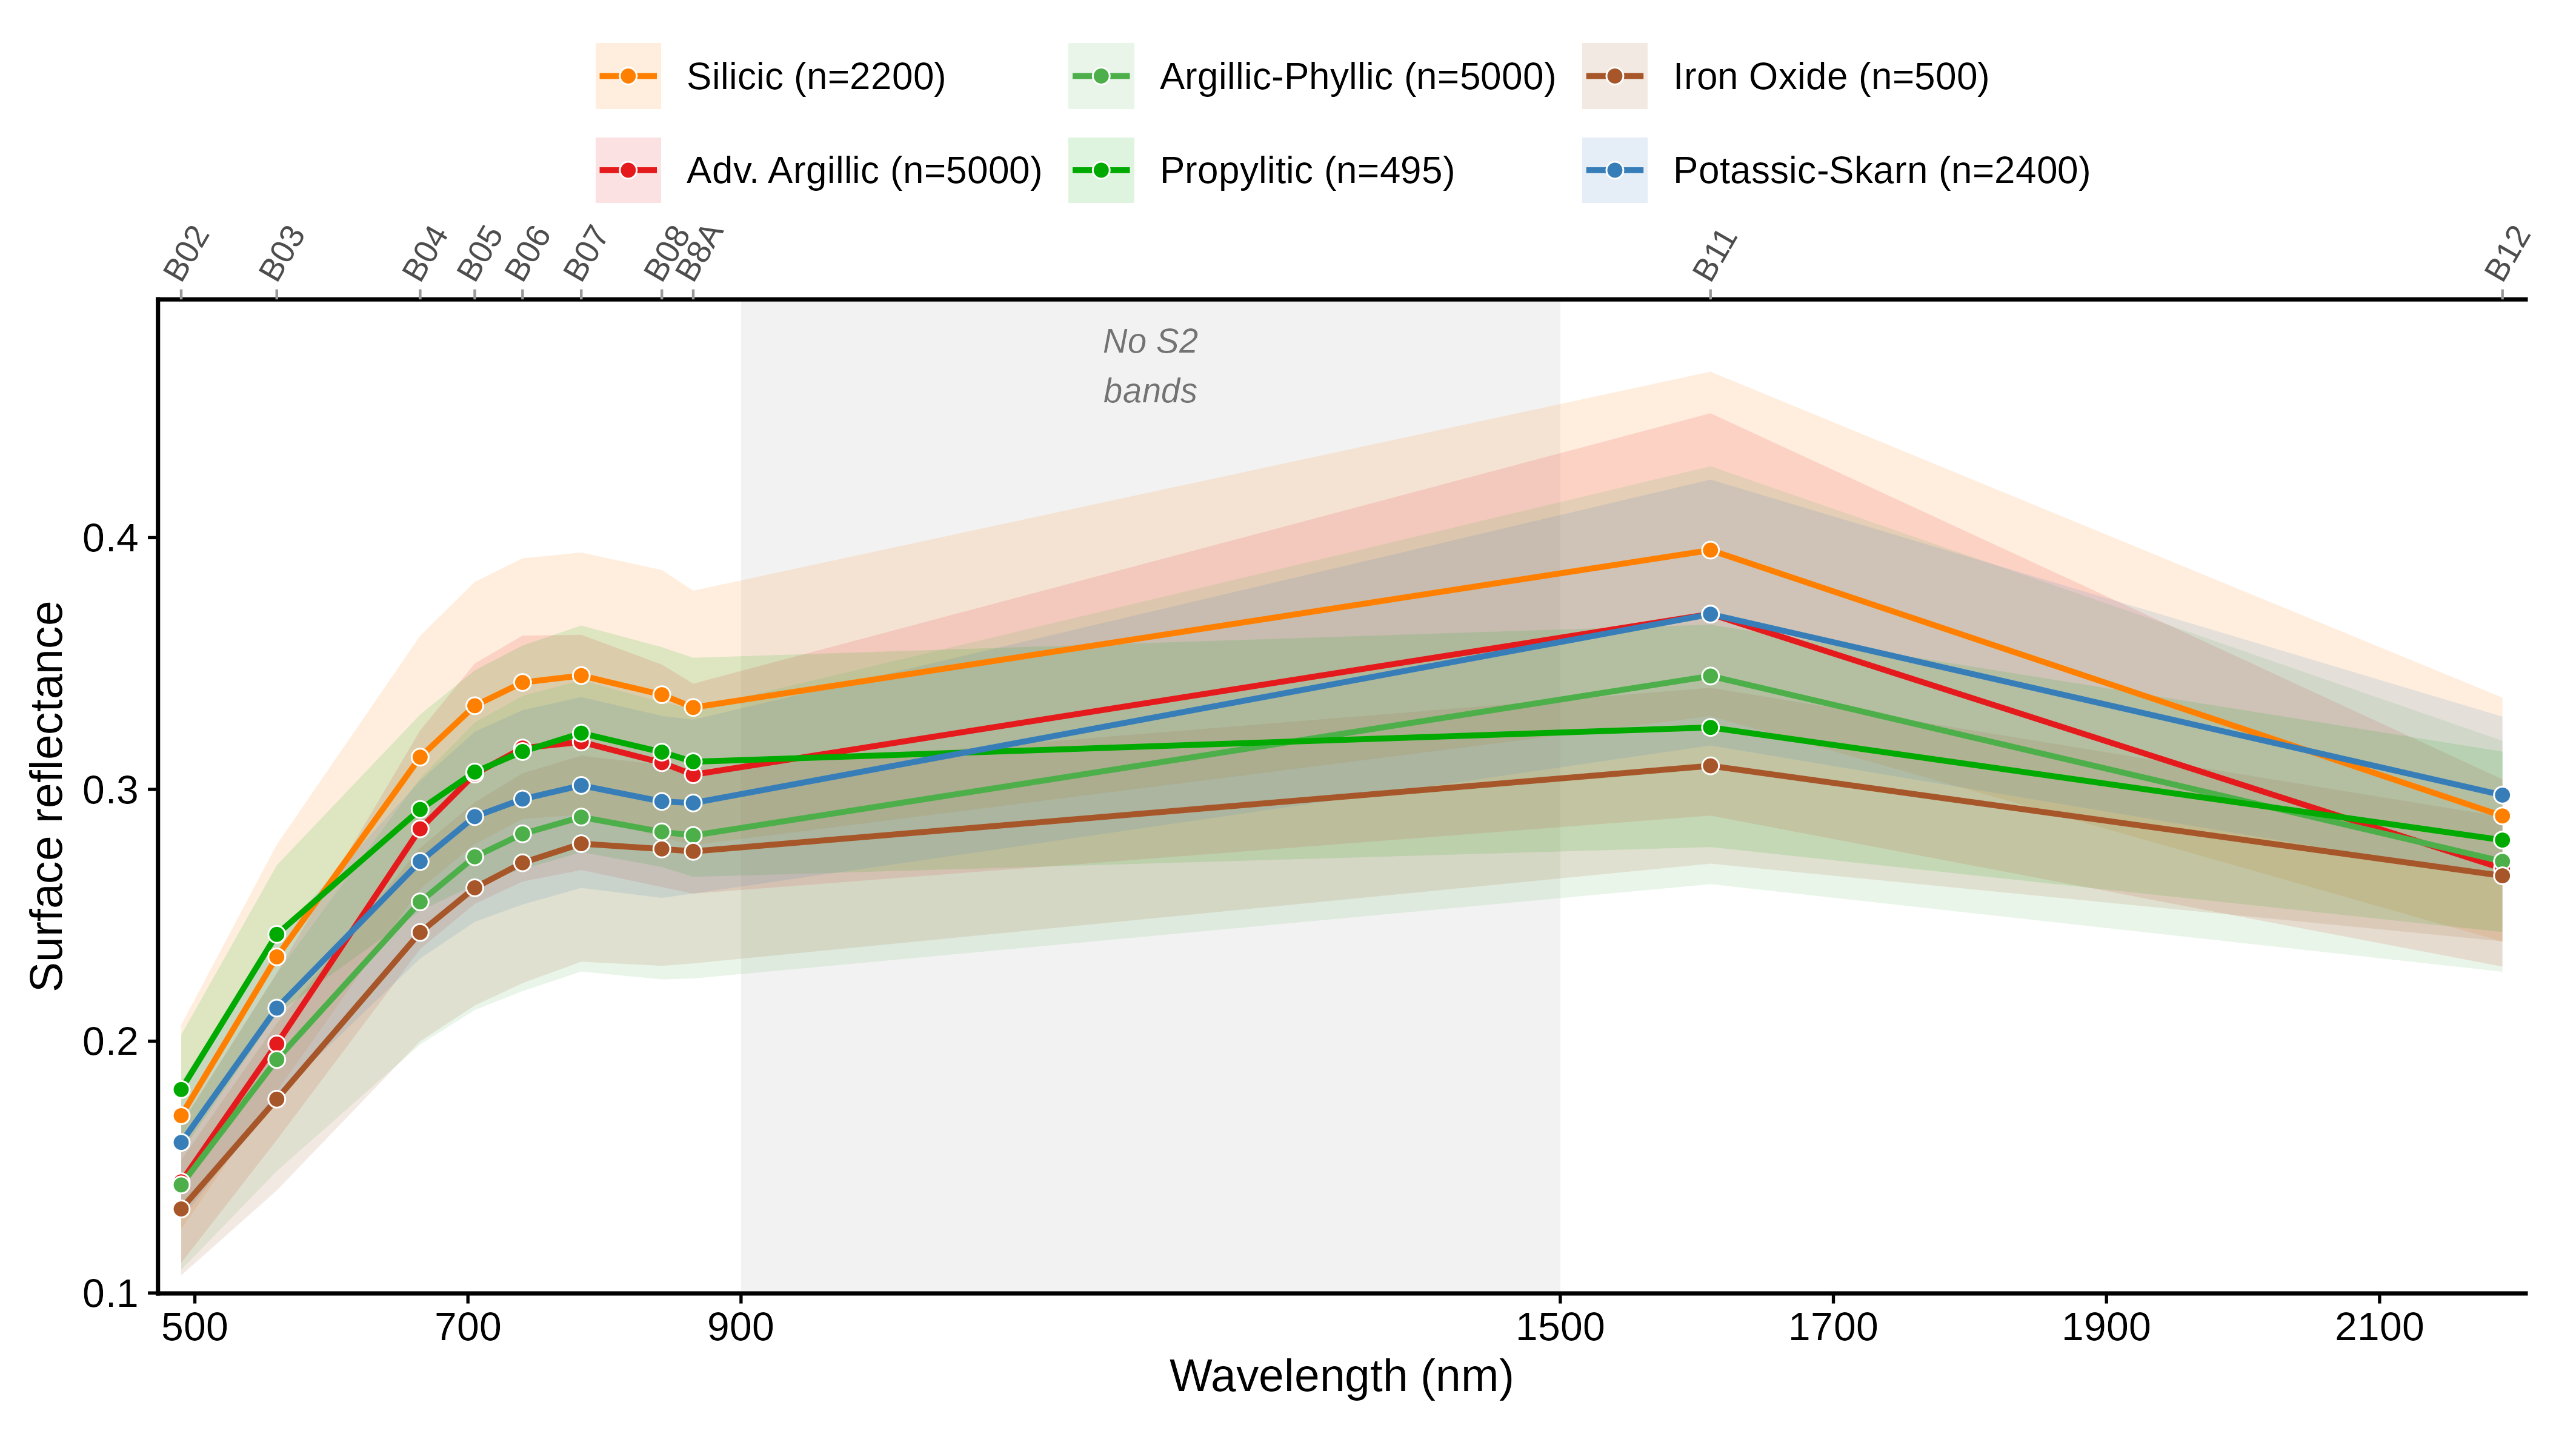
\includegraphics[width=\textwidth]{../figures/spectral_profiles.png}
\caption{Mean spectral profiles by alteration class from Sentinel-2 L2A surface reflectance (Region~III, Maricunga). Solid lines represent class means; shaded areas indicate the interquartile range (Q25--Q75). The spectral gap between \SIrange{900}{1500}{\nano\meter} corresponds to wavelengths not covered by Sentinel-2 bands. Note the distinct separation in the SWIR region (B11, B12) and the Red Edge (B05--B07).}
\label{fig:spectral_profiles}
\end{figure*}

\subsection{Symbolic Regression Framework}
\label{sec:sr_framework}

Symbolic regression was performed using PySR \citep{Cranmer2023}, which implements a multi-population evolutionary algorithm interfacing with the Julia-based SymbolicRegression.jl engine (initial discovery with v0.18; the nested cross-validation re-runs described below used v1.5, with the discovered formula structures stable across engine versions). PySR searches the space of mathematical expressions composed of input variables (spectral bands), binary operators ($+, -, \times, \div$), unary operators ($\sqrt{\cdot}, \log, \tanh, (\cdot)^2$), and numerical constants.

We adopted a one-versus-rest (OvR) strategy: for each alteration class $c$, a binary target $y_i = \mathbf{1}[y_i = c]$ was constructed, and PySR searched for a formula $f(\mathbf{x})$ minimizing the mean squared error between $f(\mathbf{x})$ and $y$. The key hyperparameters, identical in every discovery run reported in this paper (fixed split, nested folds, Cuprite, land cover), were:

\begin{itemize}
  \item \texttt{niterations} = 100 (evolutionary generations)
  \item \texttt{populations} = 30, \texttt{population\_size} = 50
  \item \texttt{maxsize} = 15 (maximum expression tree nodes)
  \item \texttt{parsimony} = 0.004 (complexity penalty)
  \item \texttt{select\_k\_features} = 5 (candidate bands pre-selected per class)
\end{itemize}

The parameter \texttt{select\_k\_features} restricts the search to the $k$ input bands most predictive of the target (as pre-screened by PySR) rather than limiting the number of bands per formula; $k = 5$ was adopted to constrain the combinatorial search space. The discovered formulas use 1--3 bands, well below this ceiling, indicating that the constraint was not binding.

For each class, PySR returns a Pareto front of expressions trading off complexity (number of tree nodes) against loss. From that front we selected the returned expression by PySR's default \emph{score} criterion (the largest loss improvement per unit of added complexity, which favours parsimony)subject to two constraints: complexity $\leq 8$ nodes, and \emph{at least two distinct bands}. The complexity bound keeps the expression inspectable at a glance. The two-band constraint is a specificity requirement rather than an accuracy one: an expression built from a single band is, under a threshold-free evaluation such as AUC, monotonically equivalent to that raw band (a fitted additive or multiplicative constant does not change the ranking of pixels), so it performs band \emph{selection} rather than discovering a spectral contrast, and it inherits that band's confounders, most importantly a sensitivity to albedo rather than to composition. Applying the constraint changes the selected expression for two of the six classes and leaves the other four unchanged; we report its cost in Section~\ref{sec:q1_standalone_discovered}. Throughout the paper we refer to the resulting class-targeted features as SR-1 through SR-6 (in the class order of Table~\ref{tab:classes}); we emphasize that these are \emph{class-discriminative features}, optimized to separate labeled classes under Sentinel-2's band configuration, not mineral-diagnostic identifiers.

Two evaluation designs with different purposes are used. For \emph{standalone index evaluation} (Q1), the Region~III subsample was split into a 70\% discovery partition and a 30\% locked hold-out (stratified, fixed seed) before running PySR; all searches ran exclusively on the discovery partition, and the locked hold-out was used only for the unbiased standalone AUC values reported in Section~\ref{sec:results}. For \emph{downstream classifier evaluation} (Q2--Q3), a fixed split is insufficient: the discovered formulas are the feature-generation stage of the classification pipeline, so any pixel used to select their bands, structure, or constants must be excluded from classifier test sets. We therefore evaluate the complete pipeline under \emph{nested cross-validation}: within each of five outer folds, PySR discovery is re-run from scratch on the outer training partition only, the resulting formulas generate features for that fold, and the outer test partition (never seen by discovery)is used solely for evaluation (Section~\ref{sec:validation}). The Cuprite external validation provides an additional, geologically independent evaluation at a site where discovery is likewise performed locally.

\subsection{Evaluation Metrics}

Each discovered index was evaluated as a continuous score for one-versus-rest binary classification. Performance was measured by:

\begin{itemize}
  \item \textbf{Area Under the ROC Curve (AUC)}: Threshold-independent measure of discrimination. Both the original score and its negation were tested, retaining the higher AUC (to accommodate both direct and inverse relationships).
  \item \textbf{Best F1 Score}: The maximum F1 score across 50 equally spaced thresholds spanning the score range.
\end{itemize}

\subsection{Comparison Methods}

We compared the SR-discovered indices against:

\begin{enumerate}
  \item \textbf{Classical spectral indices} adapted from the ASTER literature to Sentinel-2 bands:
  \begin{itemize}
    \item Clay Ratio: $B_{11}/B_{12}$ \citep{Ninomiya2005}
    \item Iron Oxide: $B_{04}/B_{02}$ \citep{Sabins1999}
    \item Ferrous: $B_{12}/B_{8A}$
    \item Alunite Index: $(B_{11}-B_{12})/(B_{11}+B_{12})$
    \item OH Minerals: $B_{02}/B_{11}$
    \item Silica Index: $B_{12}/B_{11}$
    \item NDVI: $(B_{8A}-B_{04})/(B_{8A}+B_{04})$
  \end{itemize}
  \item \textbf{Random Forest (RF)} with 200 trees, max depth 15, balanced class weights, using all 10 spectral bands. Evaluated via 5-fold stratified cross-validation.
\end{enumerate}

\subsection{SR-Informed Ensemble Classification}
\label{sec:ensemble}

Beyond their use as standalone indices, the SR-discovered formulas can serve as engineered features for downstream classifiers. We evaluated this by training Random Forest classifiers on different feature spaces derived from spectral indices:

\begin{enumerate}
  \item \textbf{RF(10 raw bands)}: All 10 Sentinel-2 bands as input, the conventional approach.
  \item \textbf{RF(6 SR indices)}: The six SR-discovered formulas computed from the raw bands, used as the sole input features.
  \item \textbf{RF(6 SR + $k$ low-correlation bands)}: SR features augmented with raw bands that have low Pearson correlation ($|r| < 0.70$) with all SR indices, to capture complementary information.
  \item \textbf{RF(7 classical indices)}: Seven classical ratio-based indices as input.
  \item \textbf{RF(6 SR + 7 classical)}: All SR and classical indices combined.
\end{enumerate}

The rationale is twofold: if RF trained on SR features approaches RF trained on raw bands, SR has compressed the spectral information into a smaller, interpretable feature space with quantifiable loss; and if adding SR features to the classical set outperforms the raw bands, the discovered features carry discriminative information that neither the raw bands nor expert-designed ratios expose to the classifier as effectively.

All RF models used 200 trees, max depth 15, and balanced class weights. Feature sets involving SR formulas were evaluated under the nested protocol of Section~\ref{sec:sr_framework}: formulas re-discovered inside each outer training fold, classifiers trained on that fold and evaluated on the held-out fold. Classical indices are fixed literature formulas and involve no fitting, so they introduce no leakage; the raw-band and classical-only baselines use the same outer folds for comparability.

\subsection{Validation Strategy}
\label{sec:validation}

Validation was conducted at three levels, treating the complete discovery-to-classification pipeline as a single predictive unit:

\begin{enumerate}
  \item \textbf{Intra-site (nested cross-validation)}: downstream classifiers on SR-derived features were evaluated with five-fold nested cross-validation under two outer-fold definitions: (a) \emph{stratified} folds at the pixel level, and (b) \emph{polygon-disjoint} folds, where GroupKFold(5) group IDs were reconstructed from pixel coordinates via DBSCAN clustering at $\approx \SI{110}{\meter}$ (below typical inter-polygon distance, above the \SI{20}{\meter} pixel size), yielding 3{,}828 spatial clusters. We refer to these as spatial clusters rather than polygons, since their correspondence to the original mapped polygons has not been individually validated; their purpose is to guarantee that spatially contiguous pixel groups never straddle a train/test boundary, which removes the AUC inflation that pixel-level cross-validation incurs through spatial autocorrelation \citep{Ploton2020,Meyer2019}. In both schemes, PySR discovery runs exclusively inside each outer training partition, so no test pixel ever influences the selection of bands, functional structures, or fitted constants (Section~\ref{sec:sr_framework}). Standalone index AUCs (Q1) use the separate 70/30 locked hold-out design.
  \item \textbf{Intra-site (spatial block robustness)}: as an additional check on spatial autocorrelation at coarser scales, we evaluated the fixed-formula feature sets under a \emph{spatial block} GroupKFold with square blocks of \SI{1}{\kilo\meter}, \SI{2}{\kilo\meter}, \SI{5}{\kilo\meter}, and \SI{10}{\kilo\meter}, in which training and test blocks are geographically disjoint (Table~\ref{tab:spatial_robust}). These runs use the formulas from the fixed 70/30 discovery split (not nested re-discovery) and are therefore reported as a secondary, scale-sensitivity analysis rather than as primary evidence.
  \item \textbf{Cross-site}: Training on Region~III, testing on Region~IV (Coquimbo). This tests standalone index transferability within the same Andean metallogenic belt (\SI{200}{\kilo\meter} distant).
  \item \textbf{External}: 3-fold CV at Cuprite, Nevada (USA), using locally sampled training data and USGS ground truth. This tests whether the SR feature engineering equivalence (SR $\approx$ raw bands) replicates at a geologically independent site on a different continent. The reduced fold count (3 vs.\ 5) reflects the smaller number of altered pixels at Cuprite (3{,}466 vs.\ 10{,}500).
\end{enumerate}


%% ============================================================
\section{Results}
\label{sec:results}

We organize the results around four progressively stronger questions, moving from the weakest interpretation of SR (a set of standalone indices) to the strongest (a re-deployable feature engineering framework):

\begin{description}
  \item[Q1.] Can SR-derived formulas work as standalone spectral indices, and how do they compare against classical expert-designed ratios? (\S\ref{sec:q1_standalone_discovered}--\S\ref{sec:q1_binary})
  \item[Q2.] Can SR-derived features replace the raw spectral bands as inputs to a classifier with minimal loss of discriminative information? (\S\ref{sec:q2q3_feature_engineering})
  \item[Q3.] Do SR-derived and classical indices capture complementary information, such that combining them yields the strongest performance? (\S\ref{sec:q2q3_feature_engineering})
  \item[Q4.] Does the feature engineering pattern (SR $\approx$ raw bands, best with SR $+$ classical) replicate at geologically independent sites? (\S\ref{sec:cuprite_results})
\end{description}

Throughout, we distinguish between \emph{formula transferability} (whether a specific discovered expression remains effective at a new site) and \emph{method transferability} (whether the SR discovery framework itself consistently yields compact and effective features when re-applied under new conditions). The first is a property of individual indices and is expected to vary by class and site; the second is the primary claim of this work, directly tested by Q4.

\subsection{Q1: Discovered formulas as standalone indices}
\label{sec:q1_standalone_discovered}

Table~\ref{tab:sr_formulas} presents the SR-discovered indices for each alteration class, selected from the Pareto front at the optimal complexity--accuracy trade-off (Fig.~\ref{fig:pareto}).

\begin{table}[h]
\centering
\caption{SR-discovered spectral indices for each alteration class. Complexity is the number of expression tree nodes. AUC values are one-versus-rest on the locked 30\% held-out subset of Region~III (intra-site, unseen during PySR discovery) and on Region~IV (cross-site). Formulas were selected from each Pareto front by PySR's score criterion under two constraints: complexity $\leq 8$ nodes and at least two distinct bands (Section~\ref{sec:sr_framework}). ``n.a.'' indicates that the class is not mapped in the Region~IV ground truth, which distinguishes only four alteration classes (Section~\ref{sec:study_areas}), so no cross-site value can be computed for it.}
\label{tab:sr_formulas}
\begin{tabular}{llccccc}
\toprule
Class & Formula & Compl. & Loss & \multicolumn{2}{c}{AUC} & Bands \\
\cmidrule(lr){5-6}
 & & & & Intra & Cross & \\
\midrule
Silicic & $B_{03}^2 / B_{12}$ & 4 & 0.115 & 0.65 & 0.83 & B03, B12 \\
Adv.\ Argillic & $0.83 - B_{02}/B_{05}$ & 5 & 0.198 & 0.72 & 0.70 & B02, B05 \\
Argillic-Phyllic & $(B_{03} + 0.105)/B_{04} - 0.83$ & 7 & 0.200 & 0.65 & 0.55 & B03, B04 \\
Propylitic & $B_{03} - 0.48 \cdot B_{11}$ & 5 & 0.029 & 0.91 & 0.82 & B03, B11 \\
Iron Oxide & $(\sqrt{B_{12}} - B_{11})^2$ & 5 & 0.030 & 0.74 & n.a. & B11, B12 \\
Potassic-Skarn & $B_{03} \cdot B_{12} / B_{07}^2 - 0.45$ & 8 & 0.115 & 0.77 & n.a. & B03, B07, B12 \\
\bottomrule
\end{tabular}
\end{table}

Several patterns emerge. The propylitic index ($B_{03} - 0.48 \cdot B_{11}$) achieved the highest intra-site AUC (0.91) and maintained strong cross-site performance (0.82). The silicic index ($B_{03}^2/B_{12}$, complexity 4) transfers best of all (cross-site AUC = 0.83 against 0.65 intra-site), which is expected for a green-to-SWIR contrast: the quantity it measures is a spectral shape rather than a site-calibrated level, so it survives the change of geological context better than it separates classes within the training site. Argillic-phyllic is the weakest transferring class (0.55).

Two of the six classes (iron oxide and potassic-skarn)have no cross-site value, because the Region~IV ground truth distinguishes only four alteration classes (Section~\ref{sec:study_areas}) and does not map those two. Their transferability is therefore untested here, and the Cuprite experiments (Section~\ref{sec:cuprite_results}) provide the only external evidence available for the framework.

All discovered formulas use at most three bands and have complexity $\leq 8$, making them trivially computable in any raster calculator, and each combines at least two distinct bands by construction (Section~\ref{sec:sr_framework}). The preference for Red Edge and SWIR bands is consistent with mineral absorption theory.

\begin{figure*}[ht]
\centering
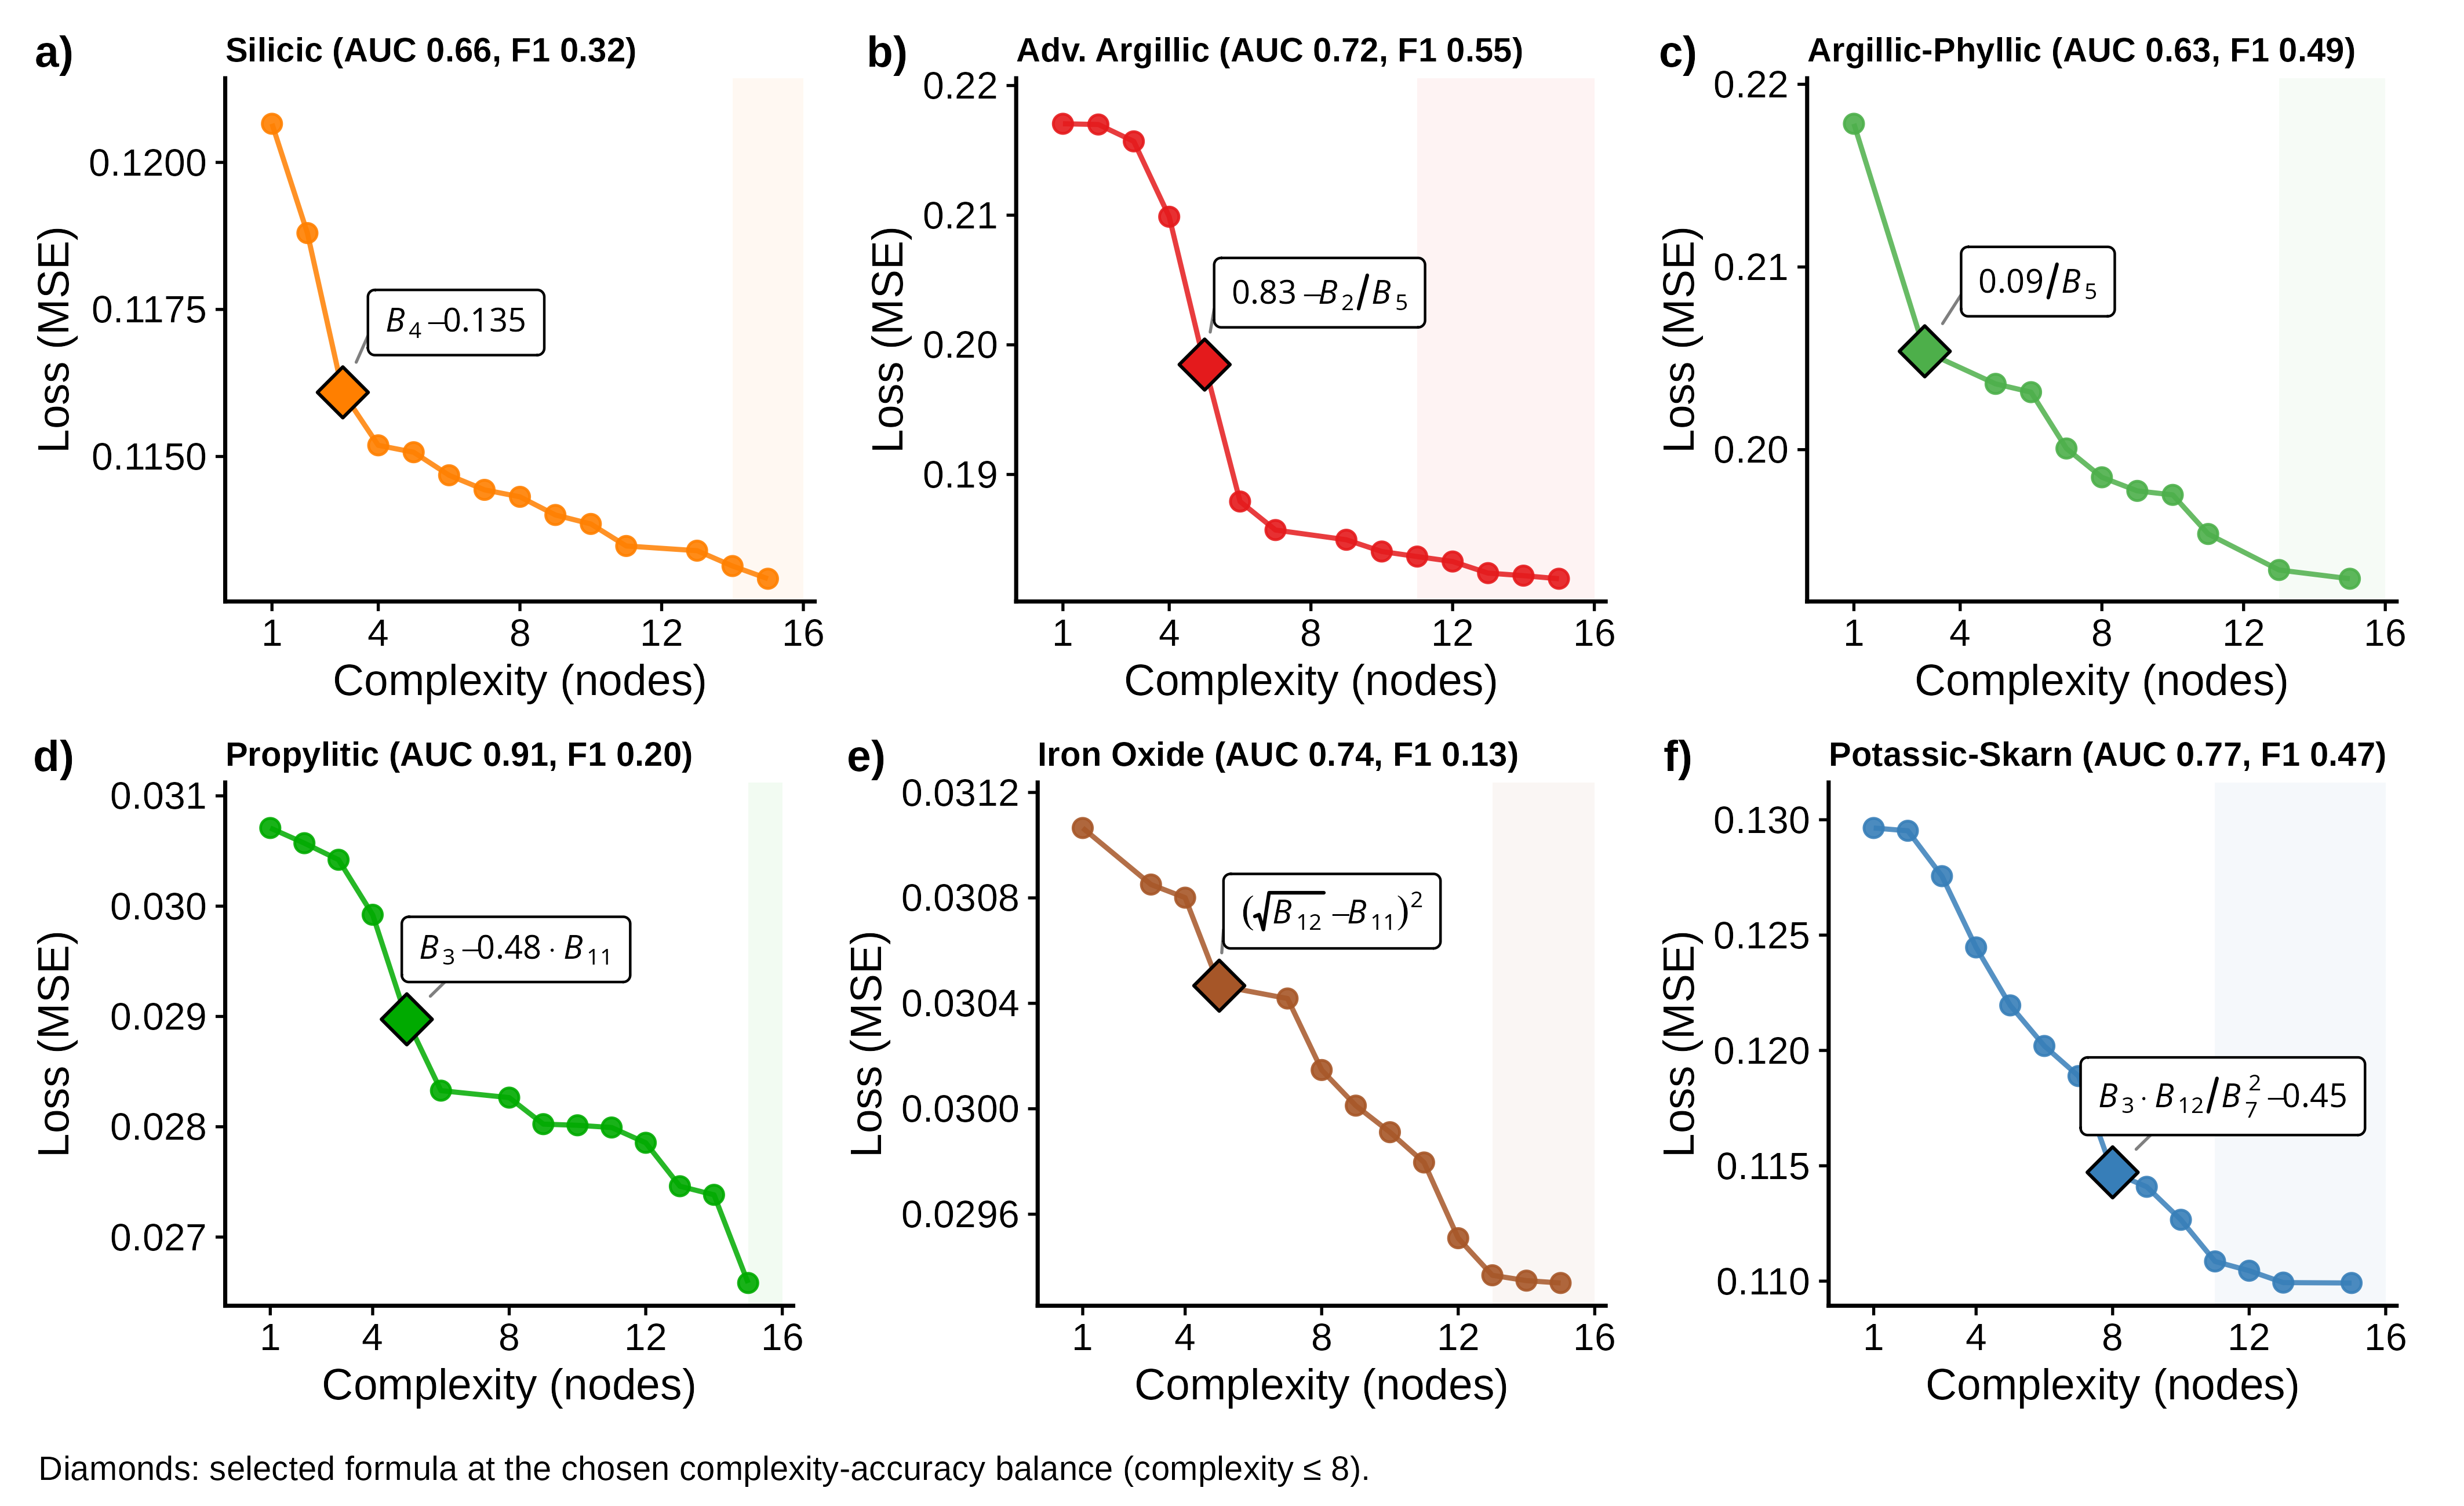
\includegraphics[width=\textwidth]{../figures/pareto_fronts.png}
\caption{Pareto fronts from symbolic regression for each alteration class, showing the trade-off between expression complexity (number of tree nodes) and loss (MSE). Stars indicate the selected formula at the optimal complexity--accuracy balance ($\leq 8$ nodes). The diminishing returns beyond complexity 8 support our selection criterion: additional nodes yield marginal loss improvements while substantially reducing interpretability.}
\label{fig:pareto}
\end{figure*}

\subsection{Q1: Standalone performance against classical indices}
\label{sec:q1_vs_classical}

Table~\ref{tab:comparison} and Fig.~\ref{fig:auc_heatmap} present the intra-site and cross-site AUC comparison between classical indices, SR-discovered indices, and the RF baseline.

\begin{table*}[ht]
\centering
\caption{AUC comparison for each alteration class (one-versus-rest). Intra-site values shown here are 5-fold stratified CV across the full Region~III dataset (mean $\pm$ std). For SR indices, applying the same closed-form formulas to the locked 30\% hold-out subset (Table~\ref{tab:sr_formulas}) yields AUCs within $\pm 0.01$ of the 5-fold values, indicating that \emph{standalone-index} optimism from the fixed discovery split is small; the downstream classifier pipeline, where discovery leakage does matter, is evaluated separately under nested CV (Table~\ref{tab:ensemble}). Cross-site: Region~III $\rightarrow$ Region~IV. DeLong test significance: $^{***}p<0.001$, $^{*}p<0.05$, n.s.\ = not significant.}
\label{tab:comparison}
\begin{tabular}{lcccccc}
\toprule
 & \multicolumn{6}{c}{Intra-site AUC (5-fold CV)} \\
\cmidrule(lr){2-7}
Method & Silicic & Adv.\ Arg. & Arg.-Phyl. & Propylitic & Iron Ox. & Pot.-Skarn \\
\midrule
Clay Ratio ($B_{11}/B_{12}$) & 0.65{\tiny$\pm$.01} & 0.63{\tiny$\pm$.01} & 0.59{\tiny$\pm$.01} & 0.72{\tiny$\pm$.01} & 0.74{\tiny$\pm$.03} & 0.60{\tiny$\pm$.01} \\
Iron Oxide ($B_{04}/B_{02}$) & 0.53{\tiny$\pm$.01} & 0.72{\tiny$\pm$.01} & 0.59{\tiny$\pm$.01} & 0.80{\tiny$\pm$.02} & 0.51{\tiny$\pm$.01} & 0.68{\tiny$\pm$.01} \\
\midrule
SR index (target class) & 0.65{\tiny$\pm$.01} & 0.72{\tiny$\pm$.01} & 0.65{\tiny$\pm$.01}$^{***}$ & \textbf{0.91}{\tiny$\pm$.01}$^{***}$ & 0.75{\tiny$\pm$.03}$^{\text{n.s.}}$ & 0.76{\tiny$\pm$.01} \\
\midrule
RF (10 bands, OvR) & \textbf{0.86}{\tiny$\pm$.01} & \textbf{0.87}{\tiny$\pm$.01} & \textbf{0.84}{\tiny$\pm$.01} & \textbf{0.99}{\tiny$\pm$.00} & \textbf{0.94}{\tiny$\pm$.01} & \textbf{0.89}{\tiny$\pm$.01} \\
\bottomrule
\end{tabular}
\end{table*}

Table~\ref{tab:comparison} presents AUC values per class on a common one-versus-rest basis, enabling fair comparison across all methods.

The SR propylitic index ($B_{03} - 0.48 \cdot B_{11}$) significantly exceeds the best classical index for its target class (AUC 0.91 vs.\ Clay Ratio 0.72; DeLong $p < 0.001$), as does the argillic-phyllic index (0.65 vs.\ 0.59; $p < 0.001$). The silicic index is statistically indistinguishable from the Clay Ratio (0.65 vs.\ 0.65; $p = 0.60$). The two-band constraint trades the nominal advantage of the unconstrained brightness detector for specificity, as discussed in Section~\ref{sec:interpretation}. For the remaining classes, SR indices match but do not significantly exceed classical indices (DeLong $p > 0.05$).

The Random Forest baseline, using all 10 bands in a one-versus-rest framework, substantially outperforms both SR and classical indices across all classes (AUC 0.84--0.99). This establishes the upper bound of what the spectral information can achieve. The SR indices sacrifice 10--30\% AUC relative to RF but gain interpretability, portability, and independence from trained model objects, properties that are critical for operational adoption.

Among the four classes for which cross-site evaluation is possible, argillic-phyllic transfers weakest (0.55) while silicic and propylitic transfer well (0.83 and 0.82). This indicates that SR-discovered indices should be validated per class before operational deployment.

\begin{figure*}[ht]
\centering
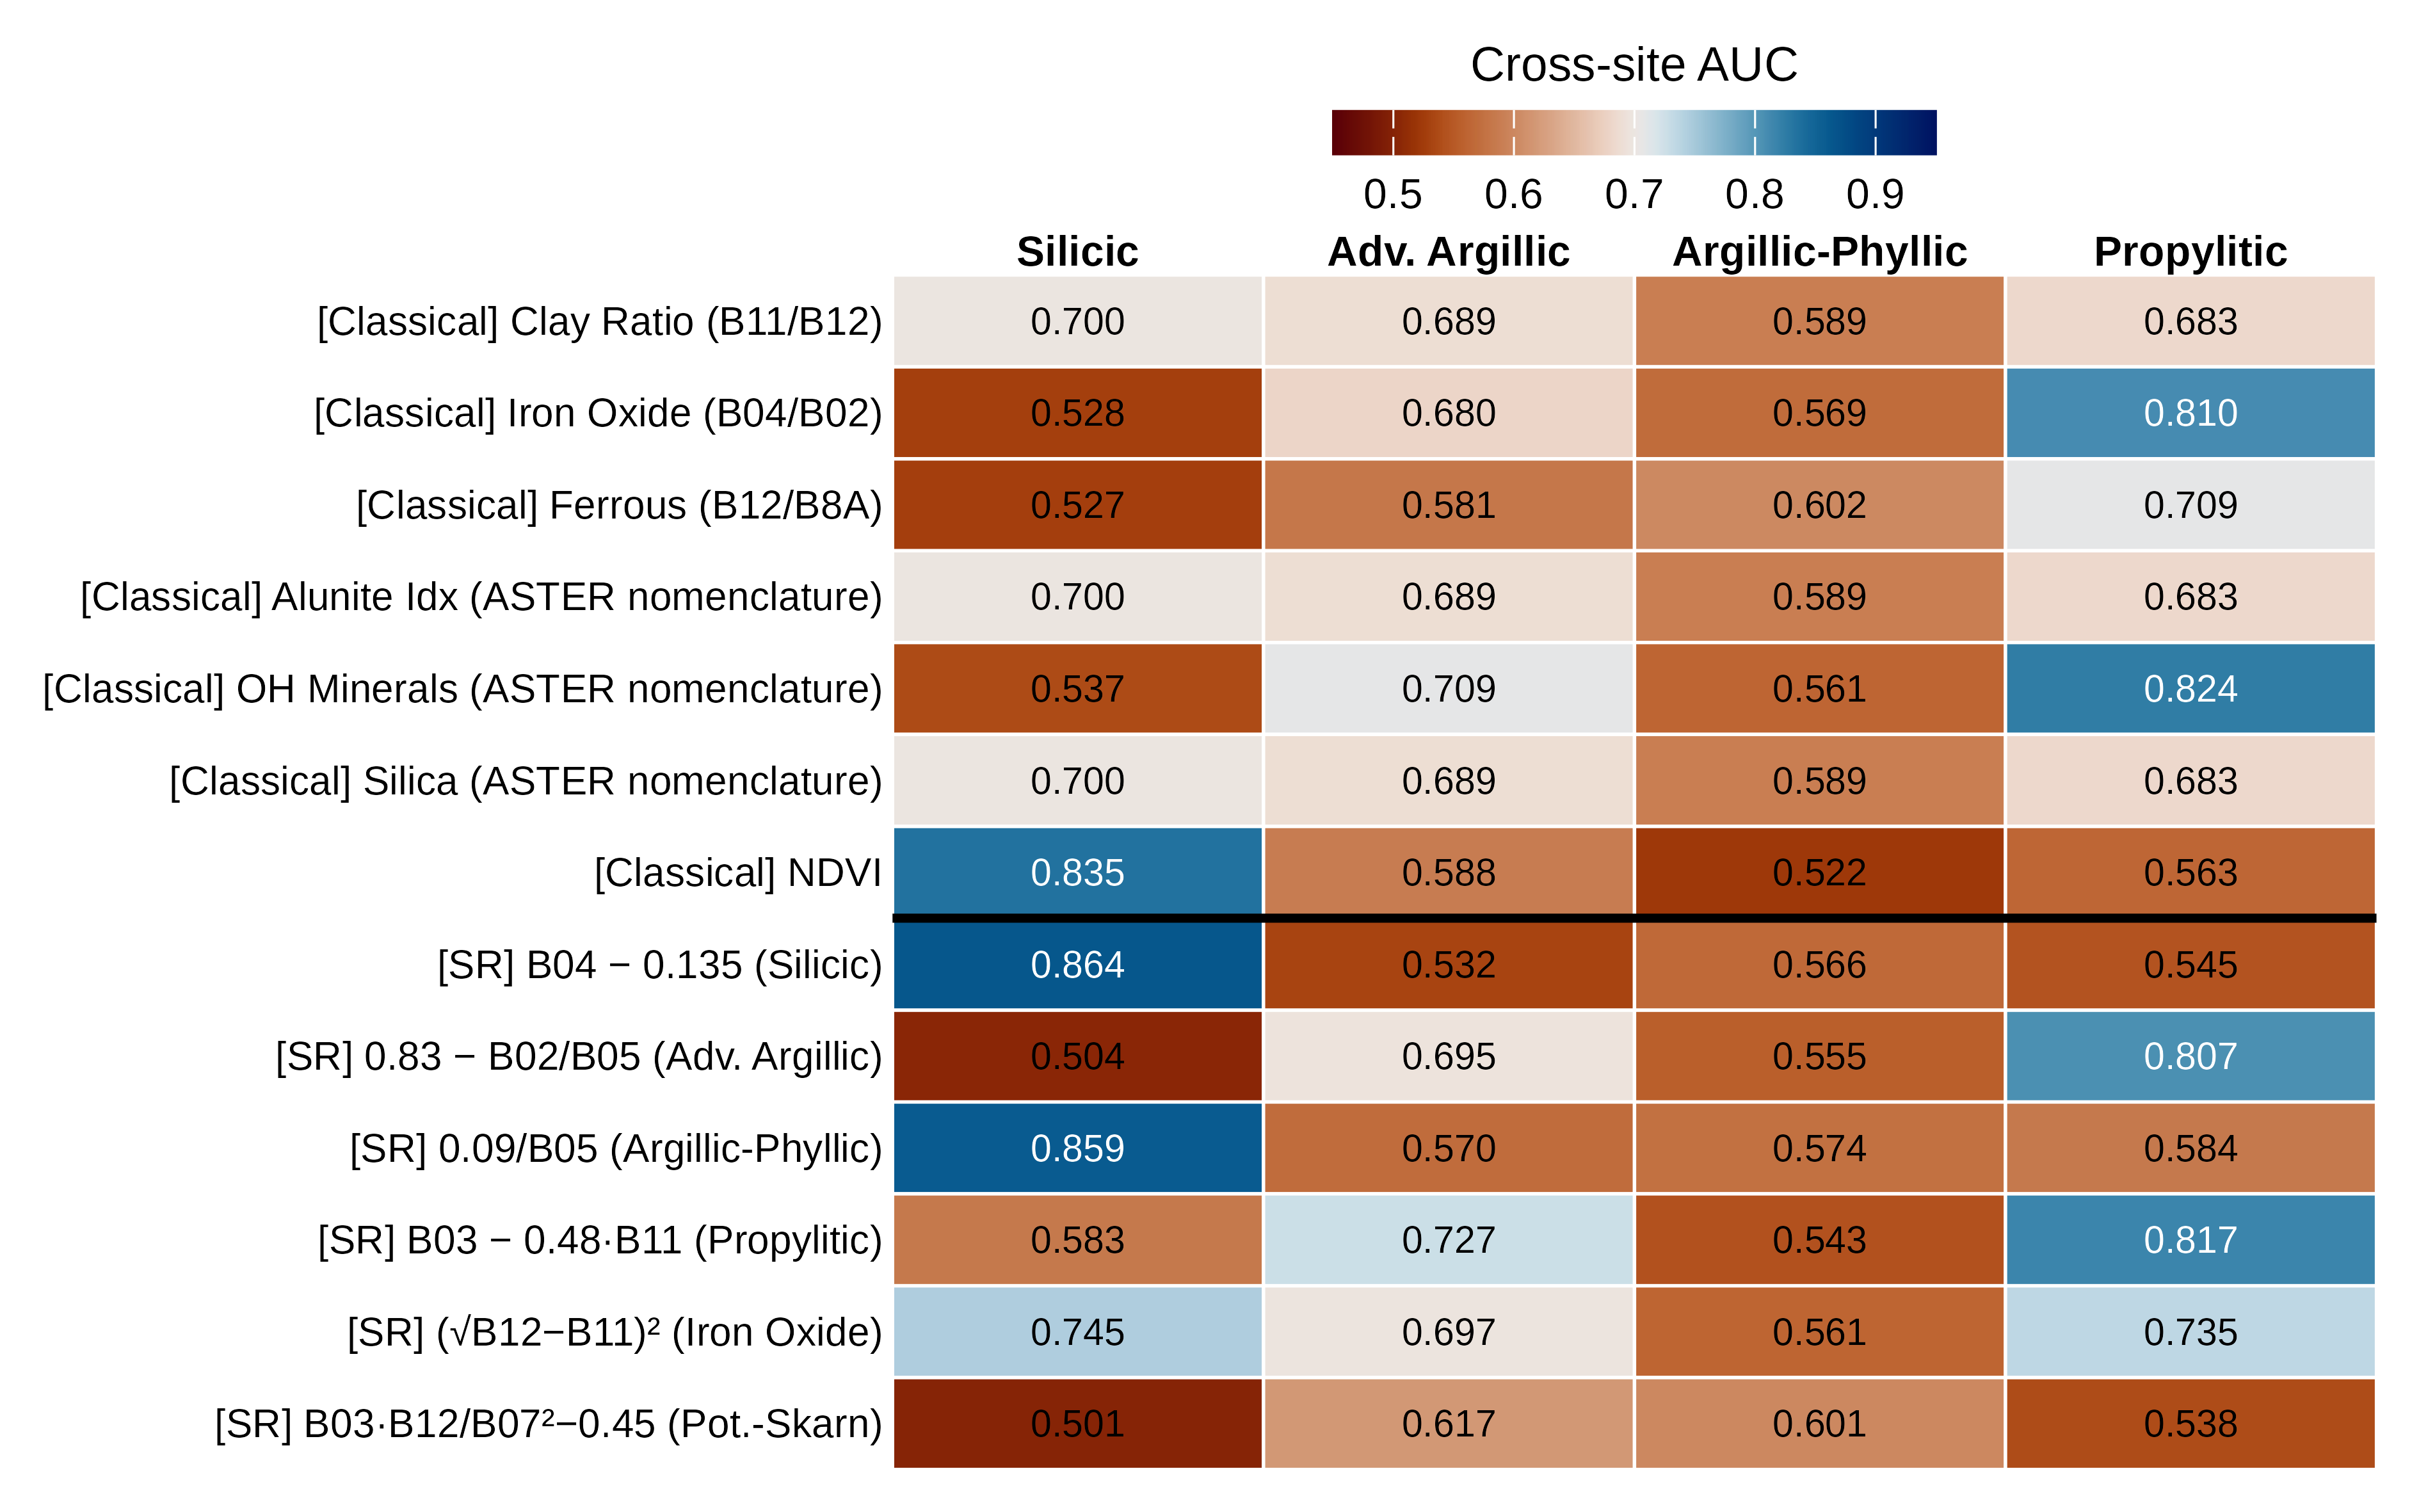
\includegraphics[width=0.85\textwidth]{../figures/auc_heatmap.png}
\caption{Cross-site validation AUC matrix (Region~III $\rightarrow$ Region~IV) for all indices and alteration classes. Upper block: classical spectral indices adapted from the ASTER literature. Lower block: SR-discovered indices. Bold values indicate AUC $>$ 0.75. The SR propylitic and silicic indices achieve the highest individual class AUCs across all methods.}
\label{fig:auc_heatmap}
\end{figure*}

% Fig. auc_comparison moved to Supplementary Material (Fig. S1)

\subsection{Q1: Binary alteration detection with a single SR formula}
\label{sec:q1_binary}

Table~\ref{tab:binary} presents the binary (altered vs.\ unaltered) detection results from the full pipeline analysis.

\begin{table}[h]
\centering
\caption{Binary alteration detection performance (altered vs.\ unaltered; $n$ = 8{,}000 per class).}
\label{tab:binary}
\begin{tabular}{lcc}
\toprule
Method & AUC & F1 \\
\midrule
SR: $(\sqrt{B_{12}} - B_{11})^2$ & 0.88 & 0.81 \\
SR: $B_{04} / 0.452$ & 0.86 & 0.79 \\
Clay Ratio ($B_{11}/B_{12}$) & 0.87 & n.a. \\
Iron Oxide ($B_{04}/B_{02}$) & 0.70 & n.a. \\
Random Forest (10 bands, 5-fold CV) & \textbf{0.93} & n.a. \\
\bottomrule
\end{tabular}
\end{table}

The SR-discovered SWIR Alteration Index $(\sqrt{B_{12}} - B_{11})^2$ achieves AUC = 0.88 for binary detection, competitive with the classical Clay Ratio (0.87) and approaching the RF upper bound (0.93). This single formula captures the general spectral deviation that alteration minerals produce in the SWIR region, regardless of specific alteration type.

Taken together, the Q1 experiments indicate that individual SR formulas can be competitive as class-specific and binary detectors (especially for propylitic alteration and general altered/unaltered discrimination)but their transferability varies by class (Tables~\ref{tab:sr_formulas},~\ref{tab:comparison}). The strongest contribution of SR therefore may lie not in the universality of any particular standalone formula, but in its value as a feature engineering mechanism, which is the subject of Q2.

\begin{figure*}[ht]
\centering
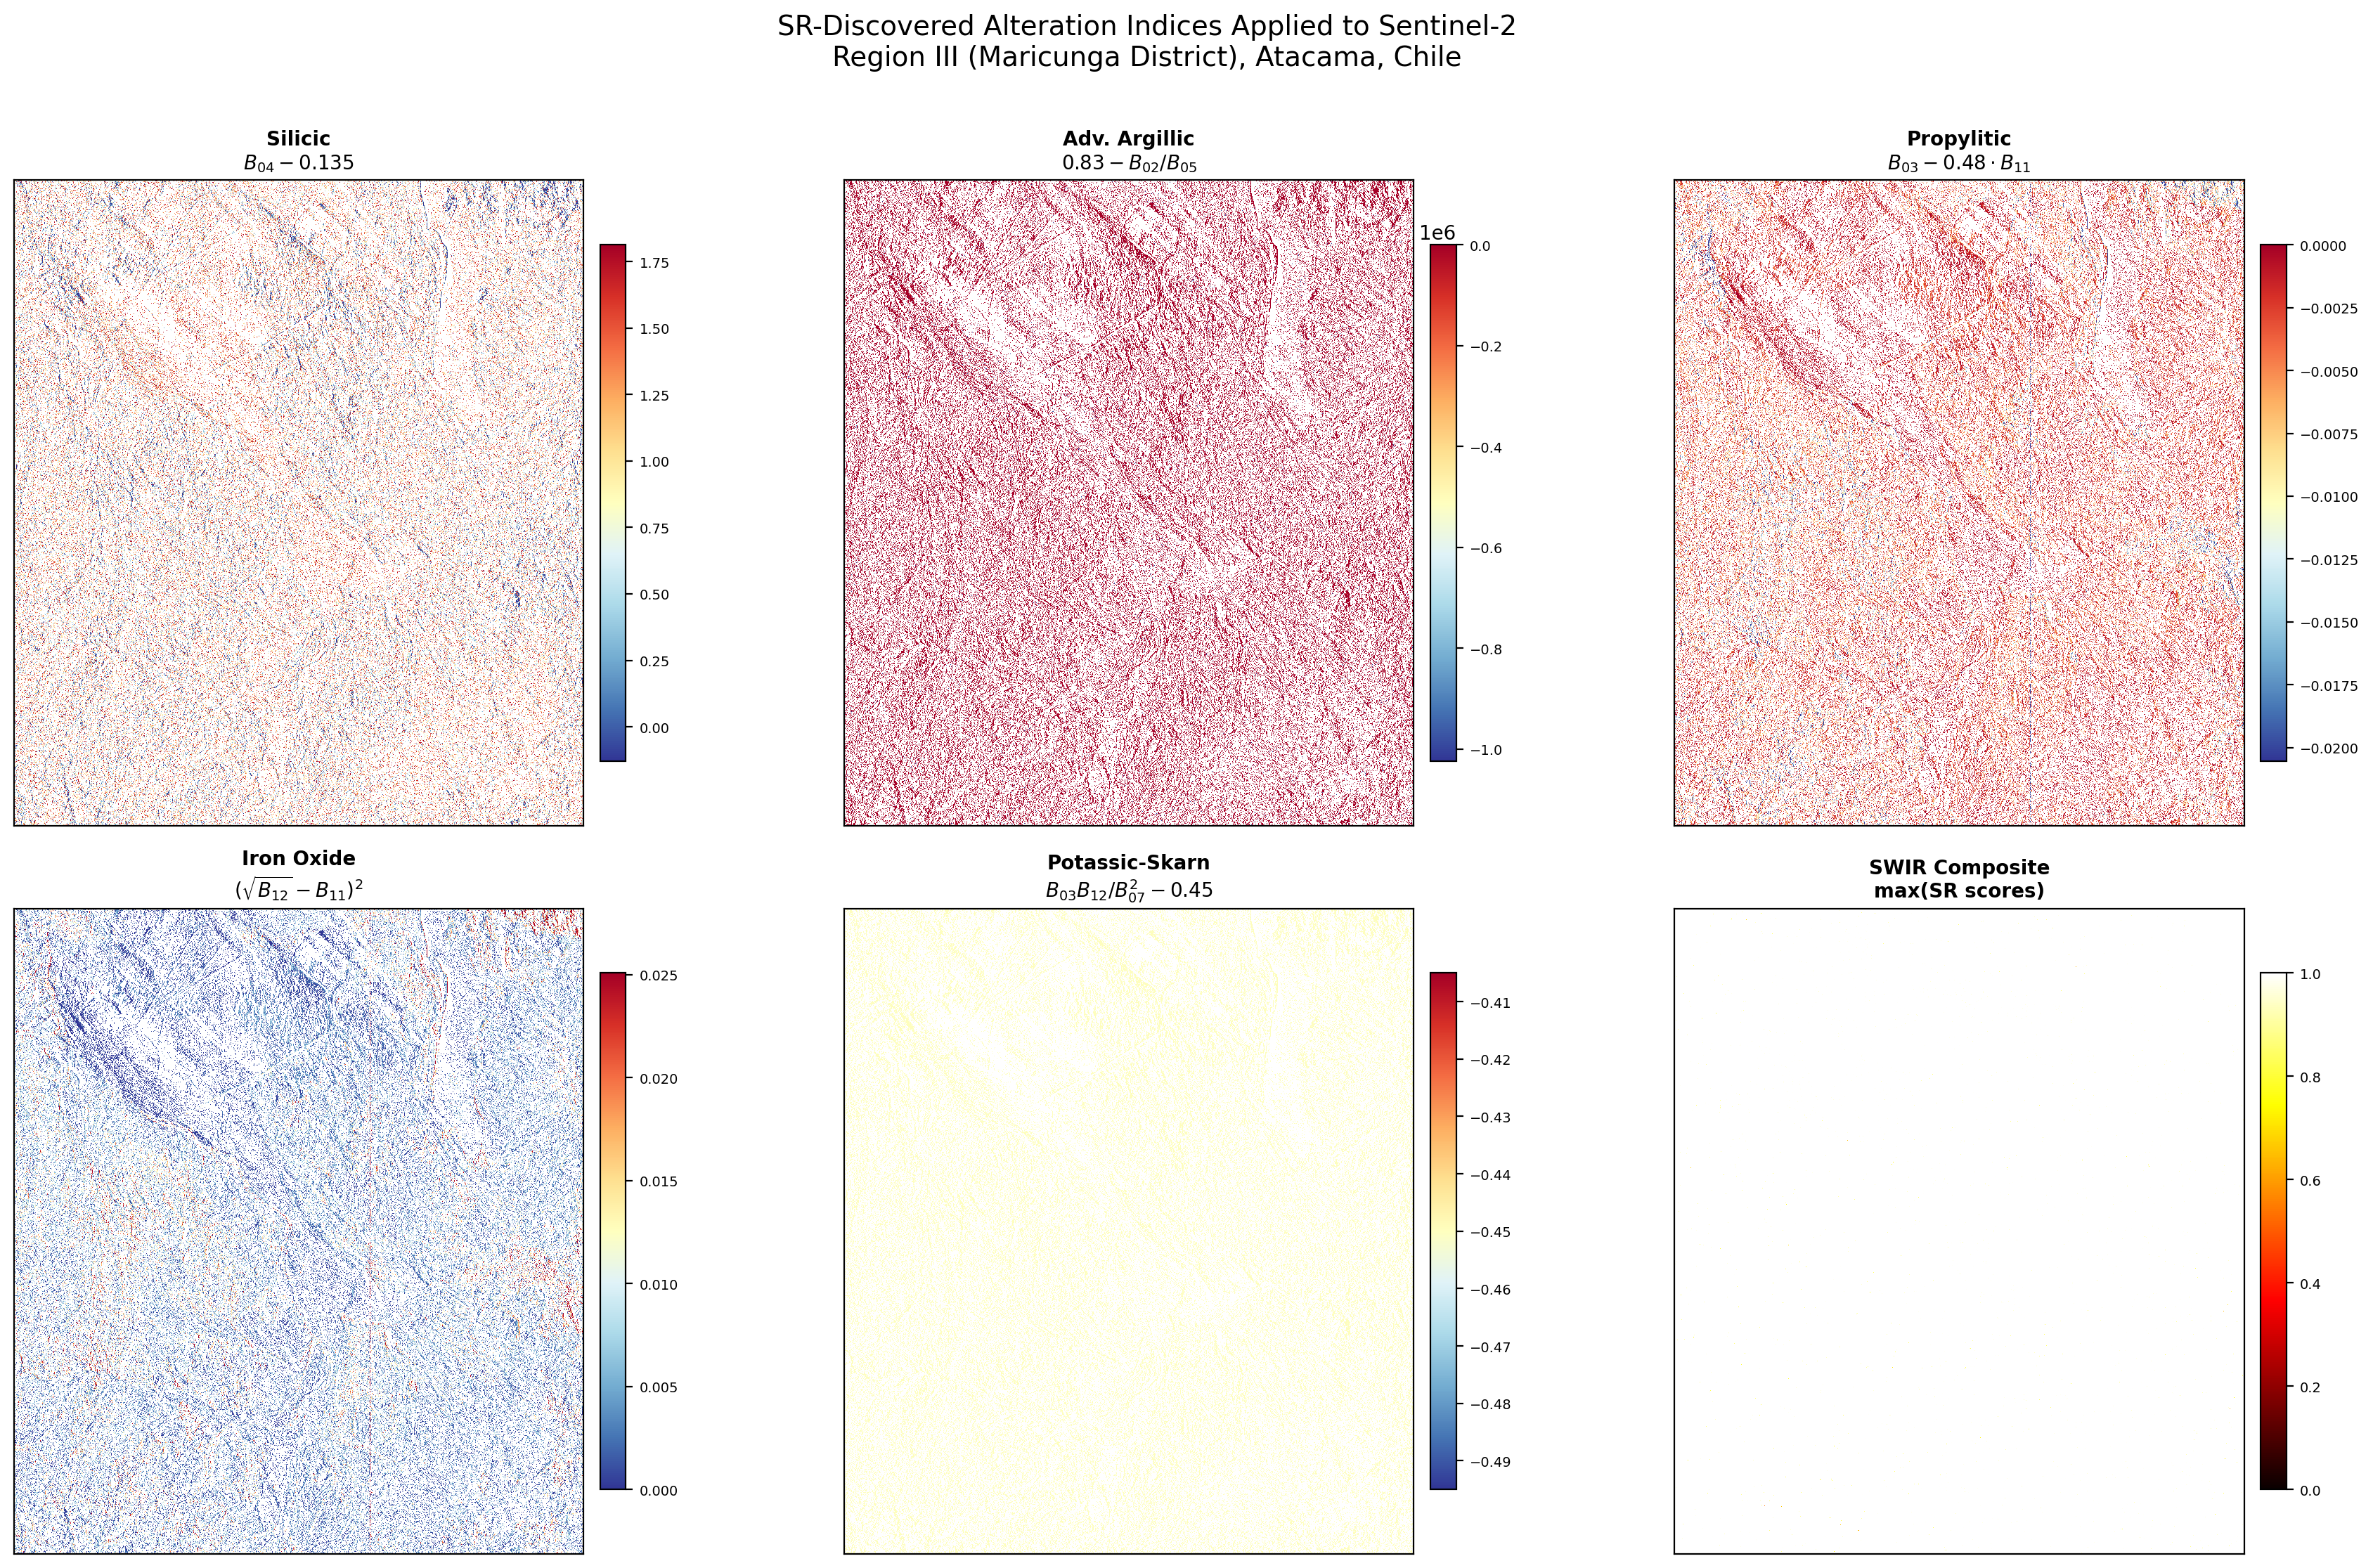
\includegraphics[width=\textwidth]{../figures/alteration_maps_sr.png}
\caption{Spatial application of SR-discovered indices to Sentinel-2 imagery over the Maricunga district (Region~III). Each panel shows one class-specific index computed from the temporal median composite (Jan--Mar 2024). The bottom-right panel shows the maximum normalized SR score across all indices, highlighting areas of strongest alteration response.}
\label{fig:alteration_maps}
\end{figure*}

\subsection{Q2 and Q3: Feature engineering equivalence and complementarity}
\label{sec:q2q3_feature_engineering}

Table~\ref{tab:ensemble} presents the central result of this study, obtained under the nested protocol of Section~\ref{sec:validation}: within each of five outer folds, PySR re-discovers all six formulas from scratch on the training partition, and every number reported here is computed on outer test pixels that never influenced discovery.

The headline finding is complementarity (Q3). A Random Forest on the six SR features plus the seven classical indices achieves a mean AUC of 0.917 under stratified nested CV, significantly exceeding the same classifier on all ten raw bands (0.899; per-fold paired difference $+0.018 \pm 0.004$, one-sided $p = 0.002$). The advantage persists under polygon-disjoint nested CV, where spatially contiguous pixel clusters never straddle a train/test boundary: 0.838 vs.\ 0.822 ($+0.016 \pm 0.005$, $p = 0.008$). The SR $+$ classical combination also outperforms the raw bands \emph{augmented} with the same classical indices (0.917 vs.\ 0.914 stratified; 0.838 vs.\ 0.832 polygon-disjoint) while using fewer features (13 vs.\ 17): the discovered formulas expose discriminative structure to the classifier more effectively than the bands they are built from.

The second finding quantifies compression (Q2). The six SR features alone retain 98.9\% of the raw-band performance under stratified nested CV (0.889 vs.\ 0.899; $\Delta = -0.011$, SE $0.004$) and 97.5\% under polygon-disjoint nested CV (0.802 vs.\ 0.822; $\Delta = -0.020$, SE $0.005$). We report the equivalence question honestly: a fold-level TOST does \emph{not} establish equivalence at $\varepsilon = 0.01$ (stratified $p = 0.62$; polygon-disjoint $p = 0.98$); the data support equivalence only at $\varepsilon = 0.02$ (stratified) and $\varepsilon = 0.03$ (polygon-disjoint). For comparison, the same experiment run with formulas from the fixed 70/30 discovery split (the design in which test pixels had influenced discovery)yields $\Delta = -0.001$ (stratified) and $-0.007$ (polygon-disjoint): the nested protocol therefore reveals a genuine discovery cost of about 0.01--0.02 AUC that the fixed-split design understates. We consider the nested figures the defensible ones and use them throughout.

The nested protocol also yields a stability result unavailable to a fixed split. The propylitic formula was rediscovered nearly verbatim across independent training partitions ($B_{03} - 0.482 \cdot B_{11}$ vs.\ the fixed-split $B_{03} - 0.48 \cdot B_{11}$), and the silicic and argillic-phyllic classes returned the same band pairs fold after fold. By contrast, the compositionally heterogeneous classes (iron oxide, potassic-skarn) produced structurally different expressions across folds, and inspection of the per-fold results shows that the 0.01--0.02 discovery cost concentrates precisely in those classes. Formula stability thus tracks the spectral coherence of the target class, evidence that the fixed-split formulas reported in Table~\ref{tab:sr_formulas} are representative outputs of the framework rather than fortunate draws.

\begin{table*}[ht]
\centering
\caption{Ensemble classification performance under leakage-free nested cross-validation (five outer folds; PySR re-run inside each training partition). All models are Random Forest (200 trees). Per-class columns are one-versus-rest AUC averaged over the stratified outer folds; the last two columns give the mean AUC under the stratified and polygon-disjoint schemes. Propylitic is excluded from the polygon-disjoint means because its pixels form a single spatial cluster (Section~\ref{sec:validation}).}
\label{tab:ensemble}
\begin{tabular}{lcccccccccc}
\toprule
 & & \multicolumn{6}{c}{Per-class AUC (stratified nested CV)} & \multicolumn{2}{c}{Mean AUC} \\
\cmidrule(lr){3-8} \cmidrule(lr){9-10}
Feature set & $n$ feat. & Silicic & Adv.Arg. & Arg.-Ph. & Propyl. & Iron Ox. & Pot.-Sk. & Stratif. & Poly.-disj. \\
\midrule
RF(10 raw bands) & 10 & 0.86 & 0.87 & 0.84 & 0.99 & 0.94 & 0.89 & 0.899 & 0.822 \\
RF(6 SR features) & 6 & 0.85 & 0.86 & 0.83 & 0.99 & 0.94 & 0.87 & 0.889 & 0.802 \\
RF(7 classical) & 7 & 0.84 & 0.85 & 0.81 & 0.99 & 0.93 & 0.86 & 0.878 & 0.789 \\
\textbf{RF(6 SR + 7 classical)} & \textbf{13} & \textbf{0.89} & \textbf{0.89} & \textbf{0.87} & \textbf{0.99} & \textbf{0.96} & \textbf{0.91} & \textbf{0.917} & \textbf{0.838} \\
RF(10 raw + 7 classical) & 17 & 0.88 & 0.88 & 0.87 & 0.99 & 0.96 & 0.90 & 0.914 & 0.832 \\
\bottomrule
\end{tabular}
\end{table*}

The SR features also outperform the classical indices as RF inputs under nesting (mean AUC 0.889 vs.\ 0.878 stratified; 0.802 vs.\ 0.789 polygon-disjoint): even paying its discovery cost, automated search produces a more discriminative six-feature set than the seven expert-designed ratios. The per-class pattern shows that the combination's advantage is broad rather than driven by a single class: SR $+$ classical improves on the raw bands for every class except propylitic, which is saturated near 0.99 for all feature sets.

Because the Atlas Metal\'ifero ground truth consists of field-mapped polygons, pixel-level cross-validation overestimates absolute AUC through spatial autocorrelation; the polygon-disjoint columns of Table~\ref{tab:ensemble} already account for this within the nested protocol. Table~\ref{tab:spatial_robust} adds a secondary, coarser-scale sensitivity analysis under spatial block cross-validation, computed with the fixed-split formulas.

\begin{table*}[ht]
\centering
\caption{Secondary sensitivity analysis: intra-site ensemble AUC under progressively stricter spatial cross-validation schemes and against dimensionality-reduction baselines. All models are Random Forest (200 trees) on Region~III, computed with the \emph{fixed 70/30-split formulas} (not nested re-discovery); the SR rows are therefore mildly optimistic relative to the nested protocol of Table~\ref{tab:ensemble} (by $\approx 0.01$, see text), and this table serves to quantify scale sensitivity, not as primary evidence. Polygon-disjoint uses DBSCAN-reconstructed spatial cluster IDs ($\approx \SI{110}{\meter}$, 3{,}828 groups); spatial block $d$ uses non-overlapping square blocks of side $d$. PCA and mutual-information top-6 baselines are fit within each training fold. SR consistently beats the MI top-6 baseline, while PCA(6) achieves higher absolute AUC at the cost of interpretability (see text).}
\label{tab:spatial_robust}
\begin{tabular}{lccccc}
\toprule
 & \multicolumn{5}{c}{Mean AUC under validation scheme} \\
\cmidrule(lr){2-6}
Feature set & Pixel 5-fold & Polygon-disj.\ & Block \SI{1}{\kilo\meter} & Block \SI{5}{\kilo\meter} & Block \SI{10}{\kilo\meter} \\
\midrule
RF(10 raw bands)             & 0.899 & 0.822 & 0.842 & 0.707 & 0.686 \\
RF(6 SR indices)             & 0.898 & 0.815 & 0.839 & 0.702 & 0.702 \\
RF(7 classical)              & 0.878 & 0.789 & 0.822 & 0.683 & 0.674 \\
\textbf{RF(6 SR + 7 classical)} & \textbf{0.920} & \textbf{0.839} & \textbf{0.862} & \textbf{0.719} & \textbf{0.708} \\
\midrule
\textit{Dimensionality-reduction baselines:} & & & & & \\
RF(PCA 6 components)          & 0.934 & 0.863 & n.a. & 0.747 & n.a. \\
RF(MI top-6 bands)            & 0.841 & 0.763 & n.a. & 0.680 & n.a. \\
\midrule
$\Delta$(SR $-$ raw)                    & $-0.001$ & $-0.007$ & $-0.003$ & $-0.005$ & $+0.016$ \\
$\Delta$(SR $-$ classical)              & $+0.019$ & $+0.026$ & $+0.017$ & $+0.019$ & $+0.028$ \\
$\Delta$(SR $-$ PCA)                    & $-0.037$ & $-0.049$ & n.a.      & $-0.045$ & n.a.      \\
$\Delta$(SR $-$ MI top-6)               & $+0.056$ & $+0.052$ & n.a.      & $+0.022$ & n.a.      \\
\bottomrule
\end{tabular}
\end{table*}

Three conclusions follow. First, as expected, absolute AUC decreases under spatial schemes, from 0.899 (pixel CV) to 0.822 (polygon-disjoint) and down to 0.686 (\SI{10}{\kilo\meter} blocks): the pixel-level estimate is inflated by spatial autocorrelation, consistently with prior work in geological remote sensing \citep{Ploton2020}. Second, comparing the fixed-split rows of Table~\ref{tab:spatial_robust} with the nested results of Table~\ref{tab:ensemble} isolates the discovery-leakage effect at matching schemes: the fixed-split design yields $\Delta(\mathrm{SR}-\mathrm{raw}) = -0.001$ (pixel) and $-0.007$ (polygon-disjoint), versus $-0.011$ and $-0.018$ under nested re-discovery. The two relative findings of this paper are nevertheless scheme-independent: SR features beat classical indices, and SR $+$ classical remains the best feature set, under every validation scheme tested. We treat the absolute pixel-level AUCs as upper bounds and Cuprite (Section~\ref{sec:cuprite_results}) as the primary out-of-site evidence of generalization. Polygon-disjoint CV cannot evaluate the propylitic class because its 495 pixels were reconstructed as a single spatially compact cluster, leaving the class absent from every test fold; propylitic therefore contributes only to the pixel- and block-level comparisons.

Third, when compared against two classical dimensionality-reduction baselines that compress the same ten bands into six features (PCA and mutual-information top-6), SR and PCA occupy distinct positions on the accuracy--interpretability trade-off rather than a strict ranking. Mutual-information band selection loses information: RF(MI top-6, 0.841 pixel) falls below even the nested RF(SR) (0.888), because MI picks highly correlated adjacent bands and misses the non-linear band combinations that SR can express. PCA(6) achieves the highest absolute AUC of any 6-feature set tested here ($0.934$ pixel, $0.863$ polygon-disjoint), exceeding RF on the ten raw bands and exceeding the nested RF(SR) by $\approx 0.05$--$0.06$; PCA is the strongest representation when downstream accuracy is the only criterion. SR(6) pays its discovery cost in exchange for features that are (i) \emph{closed-form and sensor-agnostic}, requiring no fitted transformation matrix to deploy in a new GIS; (ii) \emph{physically interpretable}, with each feature admitting a mineral-spectroscopic reading (Section~\ref{sec:interpretation}); and (iii) within 0.01--0.02 AUC of the raw bands while preserving those properties. The two methods therefore answer different questions: PCA is the appropriate choice when only the predictive distribution matters, whereas SR is the appropriate choice when the feature set itself must be auditable, transferable as algebra, and inspectable by a domain expert.

Correlation analysis revealed that all raw bands except B12 (SWIR2, \SI{2190}{\nano\meter}) have $|r| > 0.70$ with at least one SR index, explaining why raw bands add minimal information beyond the SR features. Adding B12 alone to the SR features marginally improves performance (fixed-split analysis: 0.898 $\rightarrow$ 0.902).

To verify that these results are not an artifact of the Random Forest classifier, we repeated the experiment with XGBoost \citep{Chen2016} and Support Vector Machines (SVM, RBF and linear kernels), using the fixed-split formulas (Supplementary Table~S1). The complementarity pattern holds across all four classifiers: SR $+$ classical features consistently yield the highest AUC, with the best overall result achieved by SVM-RBF (mean AUC = 0.926, BA = 0.75). Because the classifier choice is orthogonal to the discovery step, we did not repeat the full nested protocol for every classifier; the RF nested results above quantify the discovery cost that applies to all of them.

\subsection{Q4: Replication of the feature engineering pattern at Cuprite, Nevada}
\label{sec:cuprite_results}

The Cuprite site constitutes the primary independent test of method transferability in this study: a different continent, a different geological province (Basin and Range vs.\ Central Andes), and a different ground truth source (USGS ASTER-derived vs.\ SERNAGEOMIN field mapping). Two experiments were performed. The first (Table~\ref{tab:cuprite}) transfers the six \emph{Chilean} formulas to Cuprite as engineered features: RF trained on them (mean AUC = 0.942) matches RF on the 10 raw bands (0.940), and adding the classical indices achieves the highest AUC (0.952). Because these formulas were discovered on another continent, this experiment is free of any local discovery leakage by construction; what it shows is that the Chilean formulas, although site-fitted, encode band combinations that remain informative as classifier inputs at a geologically unrelated site. The second experiment (the direct test of method transferability)re-runs discovery locally and is reported below.

\begin{table}[ht]
\centering
\caption{Chilean SR formulas transferred to Cuprite, Nevada, as engineered features (3-fold CV, 20{,}000 pixels; ground truth: USGS ASTER-derived alteration map). The features are the six formulas of Table~\ref{tab:sr_formulas}, discovered in Chile and containing no information from Cuprite pixels.}
\label{tab:cuprite}
\begin{tabular}{lccccc}
\toprule
Features & mAUC & Silicic & Argillic & Phyllic & Propyl. \\
\midrule
RF(10 raw) & 0.940{\tiny$\pm$.008} & 0.97{\tiny$\pm$.00} & 0.94{\tiny$\pm$.01} & 0.95{\tiny$\pm$.01} & 0.90{\tiny$\pm$.01} \\
\textbf{RF(6 SR)} & \textbf{0.942}{\tiny$\pm$.006} & 0.97{\tiny$\pm$.00} & 0.94{\tiny$\pm$.01} & 0.95{\tiny$\pm$.01} & 0.90{\tiny$\pm$.01} \\
\textbf{RF(6SR+7cl.)} & \textbf{0.952}{\tiny$\pm$.008} & 0.97{\tiny$\pm$.00} & 0.95{\tiny$\pm$.01} & 0.96{\tiny$\pm$.01} & 0.92{\tiny$\pm$.01} \\
\bottomrule
\end{tabular}
\end{table}

Standalone SR indices (which were discovered from Chilean training data)show reduced performance at Cuprite (silicic AUC = 0.74, argillic 0.70, propylitic 0.54), as expected given the different geological context. The classical Clay Ratio ($B_{11}/B_{12}$), which does not contain fitted constants, shows strong performance at Cuprite (AUC = 0.95 for silicic), consistent with the known SWIR spectral contrast at this well-characterized site. This confirms that the standalone SR formulas are partially site-specific (due to their fitted constants), while the SR feature engineering framework generalizes.

Cross-site RF transfer trained on Chilean data and tested directly on Cuprite yielded modest AUC (0.46--0.72), confirming that the spectral characteristics of alteration differ between the Andean and Basin and Range provinces. However, the feature engineering equivalence (SR $\approx$ raw bands) holds regardless of training site, which is the methodological contribution.

\paragraph{Formulas discovered locally at Cuprite.} To make the method-transferability claim directly testable rather than merely indirect, we re-ran the identical PySR configuration on Cuprite data: the 20{,}000 sampled pixels were reduced to a stratified 15{,}000-pixel subsample and split 70/30 (fixed seed) into a 10{,}500-pixel discovery partition and a 4{,}500-pixel locked hold-out, mirroring the Chilean design (Section~\ref{sec:sr_framework}). The resulting local formulas (Table~\ref{tab:cuprite_formulas}) differ substantially from the Chilean ones in both band selection and mathematical form: they are dominated by the SWIR bands (B11, B12, B8A appear in every formula except the propylitic one), in contrast to the Chilean formulas, which rely heavily on VNIR and Red Edge. This is geologically coherent. Cuprite is the classical benchmark for advanced-argillic alteration with diagnostic SWIR absorptions (alunite at \SI{2.20}{\micro\meter}, kaolinite doublet at \SI{2.17}{\micro\meter}), whereas the Chilean Atacama site hosts a broader spectral diversity including propylitic and Fe-oxide assemblages that are partly expressed in the VNIR. SR adapts to both: at Cuprite, log($B_{11}/B_{12}$) and $B_{11} - B_{12}$ are rediscovered as optimal compact expressions, echoing but not reproducing the classical Clay Ratio.

The locally discovered formulas were then evaluated as engineered features in the leakage-free design: all classifiers were trained on the same 70\% discovery partition that produced the formulas and evaluated exclusively on the locked 30\% hold-out, which never influenced discovery. The Chilean pattern replicates quantitatively: RF on the four local SR features reaches a mean AUC of 0.920 versus 0.933 for the ten raw bands (a discovery cost of $0.014$, consistent with the 0.01--0.02 measured under nested CV in Chile)while RF on the local SR features plus the seven classical indices achieves the best result (0.939, vs.\ 0.936 for the classical indices alone and 0.933 for the raw bands). The per-class results show that the local SR cost concentrates in the propylitic class (0.846 vs.\ 0.904 for raw bands), the smallest and most heterogeneous class at this site (see below), while the three SWIR-diagnostic classes match the raw bands closely (silicic 0.963 vs.\ 0.965; argillic 0.930 vs.\ 0.933; phyllic 0.939 vs.\ 0.932).

\begin{table}[ht]
\centering
\caption{PySR formulas discovered locally at Cuprite, Nevada, using the identical configuration applied to the Chilean training site (Section~\ref{sec:sr_framework}). Compl.\ = expression-tree complexity; AUC is one-versus-rest on the 30\% locked hold-out at Cuprite. The formulas differ structurally from the Chilean ones (Table~\ref{tab:sr_formulas}) but reach substantially higher intra-site AUC, demonstrating that the SR discovery process adapts to local spectral conditions and produces site-appropriate features, the defining property of \emph{method transferability}.}
\label{tab:cuprite_formulas}
\begin{tabular}{llccc}
\toprule
Class & Formula & Compl.\ & Loss & AUC \\
\midrule
Silicic          & $\log(B_{11}/B_{12})$                    & 4 & 0.067 & \textbf{0.944} \\
Adv.\ Argillic   & $B_{11} - B_{12}$                        & 3 & 0.026 & \textbf{0.938} \\
Argillic-Phyllic & $\tanh(B_{11}) - B_{8A}$                 & 4 & 0.024 & \textbf{0.898} \\
Propylitic       & $((B_{12} - B_{08})/B_{07})^2$           & 6 & 0.025 & 0.664 \\
\bottomrule
\end{tabular}
\end{table}

Three points follow. First, comparing Tables~\ref{tab:sr_formulas} and~\ref{tab:cuprite_formulas} directly: formula transferability is weak (the Chilean silicic formula $B_{04}-0.135$ bears no structural resemblance to $\log(B_{11}/B_{12})$), but method transferability is strong: the framework, re-run locally, yields compact, interpretable formulas that outperform the transferred Chilean formulas by $+0.20$ standalone AUC or more in three of four classes. Second, the locally discovered Cuprite formulas are qualitatively consistent with prior knowledge: the SWIR difference $B_{11}-B_{12}$ and ratio $\log(B_{11}/B_{12})$ target exactly the spectral region of the diagnostic Al-OH absorptions, which is the expected mineralogical discriminator at this site. Third, the propylitic AUC at Cuprite (0.66 vs.\ 0.91 in Chile) is itself diagnostic of how the framework responds to underlying class structure. The USGS propylitic class at Cuprite merges epidote/chlorite and carbonate pixels into a broader spectral mixture than the Chilean chlorite/epidote-dominated class, and is among the smallest classes at this site (284 positives in the discovery partition). The drop in AUC is therefore an honest, automatic signal that the underlying class is compositionally heterogeneous and small in support, not a failure mode of the discovery process: rather than masking the difficulty by overfitting to the noisy class boundary, SR returns a comparatively simple expression and a degraded but truthful AUC. This is a desirable property of an automated discovery framework (one that we would expect to fail informatively when a class is poorly defined)and reinforces, rather than undermines, the case for SR as a method-transferable tool: the framework adapts to local class quality, surfacing rather than concealing differences in ground-truth coherence between sites.

\subsection{Practical application: sub-classification of undifferentiated zones}

A practical application of the discovered indices is the sub-classification of the 544 ``undifferentiated hydrothermal alteration'' polygons in the Atlas Metal\'ifero. Applying the six class-specific SR indices to 10{,}000 pixels sampled within these polygons and assigning each pixel to the class with the highest normalized score yielded the distribution shown in Table~\ref{tab:subclass}.

\begin{table}[h]
\centering
\caption{Sub-classification of undifferentiated alteration zones by SR indices and Random Forest.}
\label{tab:subclass}
\begin{tabular}{lrrrr}
\toprule
Class & \multicolumn{2}{c}{SR Indices} & \multicolumn{2}{c}{Random Forest} \\
\cmidrule(lr){2-3} \cmidrule(lr){4-5}
 & $n$ & \% & $n$ & \% \\
\midrule
Adv.\ Argillic & 7{,}450 & 74.5 & 5{,}324 & 53.2 \\
Iron Oxide & 1{,}815 & 18.2 & 269 & 2.7 \\
Potassic-Skarn & 322 & 3.2 & 907 & 9.1 \\
Propylitic & 245 & 2.5 & 239 & 2.4 \\
Silicic & 164 & 1.6 & 1{,}276 & 12.8 \\
Argillic-Phyllic & 4 & 0.0 & 1{,}985 & 19.9 \\
\bottomrule
\end{tabular}
\end{table}

Both methods agree that advanced argillic is the dominant alteration type within the undifferentiated zones (SR: 74.5\%, RF: 53.2\%), consistent with the geological expectation that argillic alteration is the most spatially extensive type in porphyry systems \citep{Sillitoe2010}. The overall pixel-level agreement between SR and RF was 51.8\%, reflecting their different classification mechanisms (threshold-based vs.\ probabilistic) rather than fundamental disagreement on the dominant patterns.

\begin{figure*}[ht]
\centering
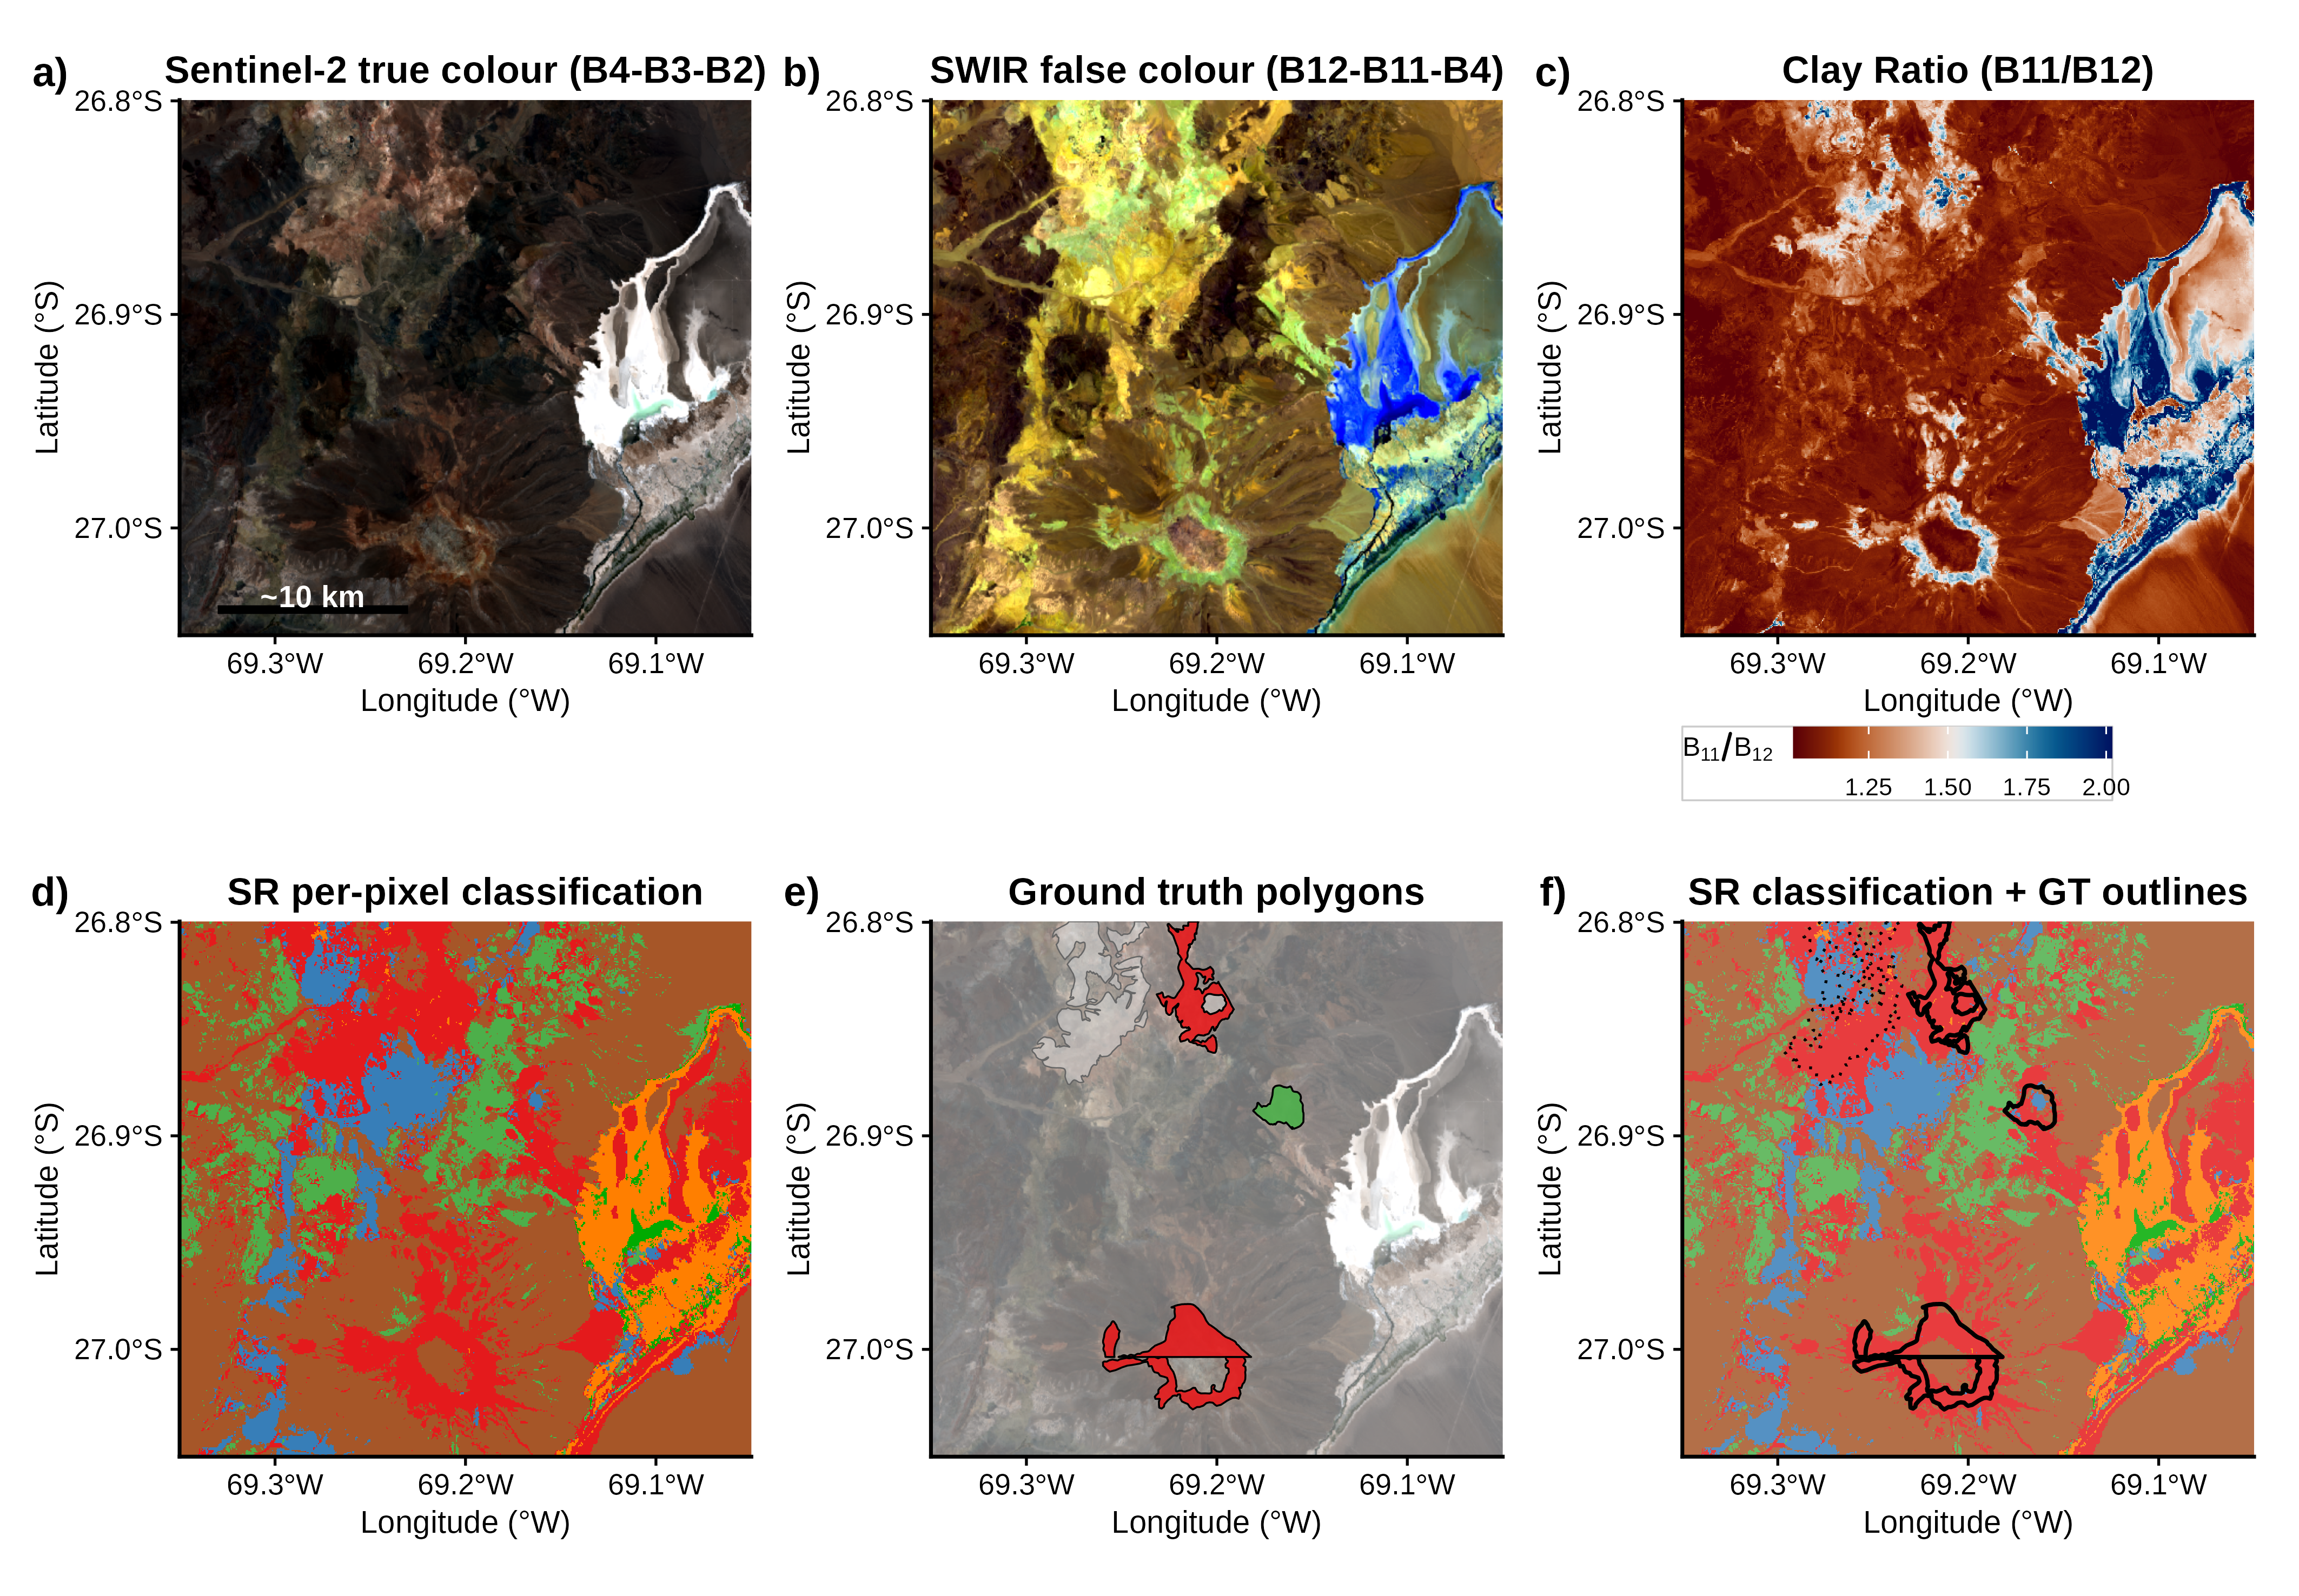
\includegraphics[width=\textwidth]{../figures/alteration_comparison.png}
\caption{Visual comparison of imagery and alteration mapping products for the Maricunga district. (a)~Sentinel-2 true color composite (B04-B03-B02). (b)~SWIR false color composite (B12-B11-B04), where alteration zones appear in distinct hues. (c)~Classical Clay Ratio ($B_{11}/B_{12}$). (d)~SR-predicted dominant alteration type, assigned per pixel as the class with the highest normalized SR index score.}
\label{fig:alteration_comparison}
\end{figure*}


%% ============================================================
\section{Physical Interpretation}
\label{sec:interpretation}

A key advantage of SR-discovered indices over black-box models is their physical interpretability. The value of the SR framework lies not only in compactness or accuracy, but in its ability to recover expressions that remain physically meaningful under the spectral constraints of Sentinel-2. Before proceeding, we restate the caveat of Section~\ref{sec:sr_framework}: these are class-discriminative features (SR-1 to SR-6), not mineral-diagnostic identifiers; the interpretations below explain why each formula separates its target class in this dataset, and correlation of a formula with a labeled class does not imply unique detection of any mineral. We analyze each formula in turn along four dimensions: the spectral contrast it encodes, the mineralogical assemblage this contrast plausibly reflects, the empirical performance observed in this study, and the residual limitation imposed by Sentinel-2's broadband SWIR configuration relative to a hyperspectral sensor (Fig.~\ref{fig:interpretation}; see also Supplementary Figs.~S1--S2 for per-class AUC bar charts and per-band boxplots).

\subsection{SR-4 (propylitic target): $B_{03} - 0.48 \cdot B_{11}$}

\emph{Spectral mechanism.} This formula encodes a contrast between Green reflectance (B03, \SI{560}{\nano\meter}) and SWIR1 (B11, \SI{1610}{\nano\meter}). The coefficient 0.48, optimized by SR to minimize MSE, effectively scales B11 to the dynamic range of B03, so that propylitic zones (high B03, moderate B11) yield positive values and unaltered rock or other alteration types yield near-zero or negative values.

\emph{Mineralogical interpretation.} The contrast is consistent with the spectral behavior of chlorite- and epidote-rich propylitic assemblages, which exhibit relatively high reflectance in the visible--NIR region but have Mg-OH and Fe-OH absorption features that reduce SWIR reflectance \citep{Hunt1977,Clark1999}. The formula captures the broader spectral shape expected from these assemblages rather than any single narrow absorption.

\emph{Performance.} Highest intra-site AUC among all discovered indices (0.91 on the locked 30\% hold-out; DeLong $p < 0.001$ against the best classical index for this class). Cross-site AUC at Region~IV remains strong (0.82), consistent with chlorite/epidote being a spectrally distinctive and regionally stable assemblage.

\emph{Sentinel-2 limitation.} The diagnostic Mg-OH absorption of chlorite and epidote lies near \SIrange{2.25}{2.35}{\micro\meter}, which falls inside B12 (\SI{2190}{\nano\meter}, \SI{180}{\nano\meter} bandwidth) rather than being resolved as a narrow feature. B11 does not sit on an absorption peak either; it simply samples the SWIR shoulder. As a consequence, the index responds to the overall Green--SWIR spectral slope rather than to a specific mineral absorption. A sensor with narrow SWIR bands (e.g., ASTER's five SWIR channels or a hyperspectral instrument) could in principle isolate those features directly, but the broadband slope captured by Sentinel-2 is already sufficient to discriminate propylitic zones from other classes in this study.

\subsection{SR-2 (advanced argillic target): $0.83 - B_{02}/B_{05}$}

\emph{Spectral mechanism.} The formula uses the $B_{02}/B_{05}$ ratio (Blue, \SI{490}{\nano\meter} over Red Edge 1, \SI{705}{\nano\meter}) to capture the spectral slope across the visible: altered surfaces show a steep increase from Blue to Red Edge (low ratio), while unaltered surfaces have a flatter response (ratio closer to 1). The additive constant 0.83, fitted by SR, simply shifts the index so that altered surfaces yield positive values.

\emph{Mineralogical interpretation.} The VNIR slope reflects the typical spectral behavior of kaolinite- and alunite-bearing surfaces, which have low Blue reflectance and increasing reflectance toward the Red Edge \citep{Clark1999}. Notably, the formula does not include B12 (where the diagnostic Al-OH absorption of kaolinite and alunite actually resides)because the VNIR slope alone carries enough class-discriminative signal at Sentinel-2 resolution. This is a non-obvious discovery: domain intuition would place the index in the SWIR, but SR identifies a more reliable discriminator in the VNIR for this sensor.

\emph{Performance.} AUC = 0.72 intra-site, 0.70 cross-site. Does not significantly exceed classical indices for this class (DeLong $p > 0.05$), but provides a spectrally distinct alternative anchored on VNIR rather than SWIR.

\emph{Sentinel-2 limitation.} The true diagnostic features of advanced argillic minerals are narrow Al-OH absorptions near \SI{2.17}{\micro\meter} (kaolinite doublet) and \SI{2.20}{\micro\meter} (alunite), both of which fall inside B12 (\SI{2190}{\nano\meter}, \SI{180}{\nano\meter} bandwidth) and cannot be resolved as distinct features at Sentinel-2 resolution. Hyperspectral sensors (or ASTER's narrower SWIR bands) would provide a more mineralogically specific expression. The VNIR-based formula found by SR is a sensor-adapted approximation to the underlying mineralogy rather than a direct detection of diagnostic absorptions.

\subsection{SR-5 (iron oxide target; SWIR alteration detector): $(\sqrt{B_{12}} - B_{11})^2$}

\emph{Spectral mechanism.} This non-linear combination of the two SWIR bands detects any mineral whose absorption features alter the standard $B_{11}/B_{12}$ relationship of unaltered rock. The square root compresses $B_{12}$'s dynamic range, and the squared difference amplifies both positive and negative spectral slope anomalies symmetrically, making the index a sensitive detector of deviation from baseline SWIR behavior rather than a measure of a specific slope direction.

\emph{Mineralogical interpretation.} OH-bearing minerals (clays, micas, hydrous silicates) and iron oxides both modify the $B_{11}$--$B_{12}$ relationship through absorptions in different portions of the \SIrange{1.6}{2.2}{\micro\meter} region. The symmetric formulation allows the index to respond to any alteration assemblage that breaks the unaltered rock's SWIR spectral continuum, which is why it performs well as a general altered/unaltered detector without being tied to a single mineralogy.

\emph{Performance.} Best-performing single formula for binary (altered vs.\ unaltered) detection (AUC = 0.88, F1 = 0.81; Table~\ref{tab:binary}), competitive with the classical Clay Ratio (0.87) and approaching the 10-band RF upper bound (0.93).

\emph{Sentinel-2 limitation.} With only two SWIR bands, Sentinel-2 cannot resolve the distinct absorptions between \SIrange{2.0}{2.4}{\micro\meter} that ASTER's five SWIR channels capture. The index is therefore well-suited as a binary (altered/unaltered) screening tool at Sentinel-2 resolution, but it cannot discriminate among alteration types based on SWIR features alone. This is the structural reason why class-specific indices additionally draw on VNIR and Red Edge bands.

\subsection{SR-1 (silicic target): $B_{03}^2 / B_{12}$ and the specificity constraint}

\emph{Spectral mechanism.} A contrast between squared Green reflectance (B03, \SI{560}{\nano\meter}) and SWIR2 (B12, \SI{2190}{\nano\meter}). The ratio responds to the overall VNIR-to-SWIR slope: silica-rich surfaces combine high visible reflectance with a comparatively flat, unabsorbing SWIR response, so the quotient rises. Squaring the numerator sharpens the response at the bright end without changing its direction.

\emph{Mineralogical interpretation.} Quartz-dominated silicic zones (vuggy silica, silica caps) show a relatively featureless but high-reflectance spectrum at Sentinel-2 resolution. Because the formula is a ratio rather than a level, it measures the \emph{shape} of that spectrum instead of its brightness, which is what allows it to separate silica-rich surfaces from other bright materials whose VNIR--SWIR slope differs.

\emph{Performance.} Intra-site AUC = 0.65 on the locked hold-out, and the best cross-site transfer of the whole set (0.83 at Region~IV). The reversal between the two (weaker within the training site, stronger across sites)is the signature of a shape-based rather than level-based index: it forfeits some within-site separation, which a site-calibrated brightness threshold can exploit, in exchange for a quantity that remains meaningful under a change of geological context.

\emph{Why this formula, and not the brightness detector.} Run without the two-band constraint (Section~\ref{sec:sr_framework}), PySR's score criterion returns $B_{04} - 0.135$ for this class at complexity~3: a single-band threshold on Red reflectance, monotonically equivalent to $B_{04}$ itself. Its intra-site AUC is marginally higher (0.66 versus 0.65), and it would have been the natural selection under a purely accuracy-driven rule. A specificity test against non-silicic surfaces shows why that would have been the wrong choice. Salt flats (Salar de Atacama, Salar de Uyuni), sandy desert, snow, and even unaltered rock all produce 99--100\% false-positive rates under that formula, because their Red reflectance exceeds the fitted threshold; only urban surfaces (51\% FP) and water are partially excluded. The high AUC reflects the correlation between albedo and silicic alteration \emph{within this study area}, not a mineralogical signature. The constrained selection trades $0.015$ AUC for an index that measures a spectral contrast instead of a brightness level, and that is the trade we take.

\emph{Sentinel-2 limitation.} The fundamental obstacle is not Sentinel-2-specific: the silica features that truly diagnose silicic alteration (reststrahlen bands near \SI{9}{\micro\meter}) lie in the thermal infrared, which neither Sentinel-2 nor ASTER's SWIR subsystem can sense. Without TIR information, any broadband VNIR/SWIR sensor discriminates silicic alteration only indirectly, through spectral shape. This class therefore remains the weakest-founded of the six, and we recommend pairing this index with SWIR-based ones for operational use.

\emph{A generalizable lesson.} The episode is not a single-class disclaimer but a property of the method worth stating plainly: a parsimony-driven selector is blind to specificity, and in any dataset where one class covaries strongly with a scalar proxy (here, albedo)it will preferentially return that proxy rather than a compositionally meaningful contrast. The remedy is to constrain the \emph{selection} step rather than the search, which costs nothing in search time and leaves the Pareto front intact for inspection. The minimum-two-band rule used here is the cheapest such gate. A stricter version, which we recommend where distractor surfaces can be enumerated, is a \emph{specificity gate}: before returning a formula, evaluate its response on domain-relevant distractors (salt flats, sandy desert, snow, unaltered lithologies) and reject any candidate whose false-positive rate on them exceeds a pre-set threshold (Section~\ref{sec:discussion}).

\subsection{SR-6 (potassic-skarn target): $B_{03} \cdot B_{12}/B_{07}^2 - 0.45$}

\emph{Spectral mechanism.} This three-band formula combines Green (B03), Red Edge 3 (B07, \SI{783}{\nano\meter}), and SWIR2 (B12). The $B_{12}/B_{07}^2$ ratio amplifies the SWIR-to-Red-Edge contrast, and the squared denominator makes the index particularly sensitive to variations in Red Edge reflectance. The multiplication by $B_{03}$ provides a brightness normalization factor.

\emph{Mineralogical interpretation.} Potassic alteration (biotite, K-feldspar) and calc-silicate skarn assemblages (epidote, garnet, diopside) combine Fe-bearing and Mg-bearing phases that produce comparatively weak, broad features in the VNIR and SWIR. The formula responds to a composite spectral shape rather than to a single diagnostic absorption. This compositional heterogeneity is likely why SR required a three-band, complexity-8 formula here, as opposed to the much simpler expressions for classes with cleaner spectral signatures.

\emph{Performance.} Intra-site AUC = 0.77, but cross-site AUC drops to 0.54, the weakest transferability among all discovered formulas.

\emph{Sentinel-2 limitation.} The poor cross-site performance likely has two causes. First, the potassic-skarn class groups assemblages with genuinely different spectral signatures (biotite-rich vs.\ calc-silicate-rich), so a single formula cannot be globally optimal. Second, the diagnostic features of the constituent minerals (Fe$^{2+}$ absorptions near \SI{1.0}{\micro\meter}, Mg-OH features at \SI{2.3}{\micro\meter}) either fall between Sentinel-2 bands or inside broad ones, forcing SR to rely on indirect spectral proxies that are more sensitive to site-specific lithological context than to the target mineralogy itself. This class would benefit most from hyperspectral data or from splitting into mineralogically narrower sub-classes before SR discovery.

\begin{figure*}[ht]
\centering
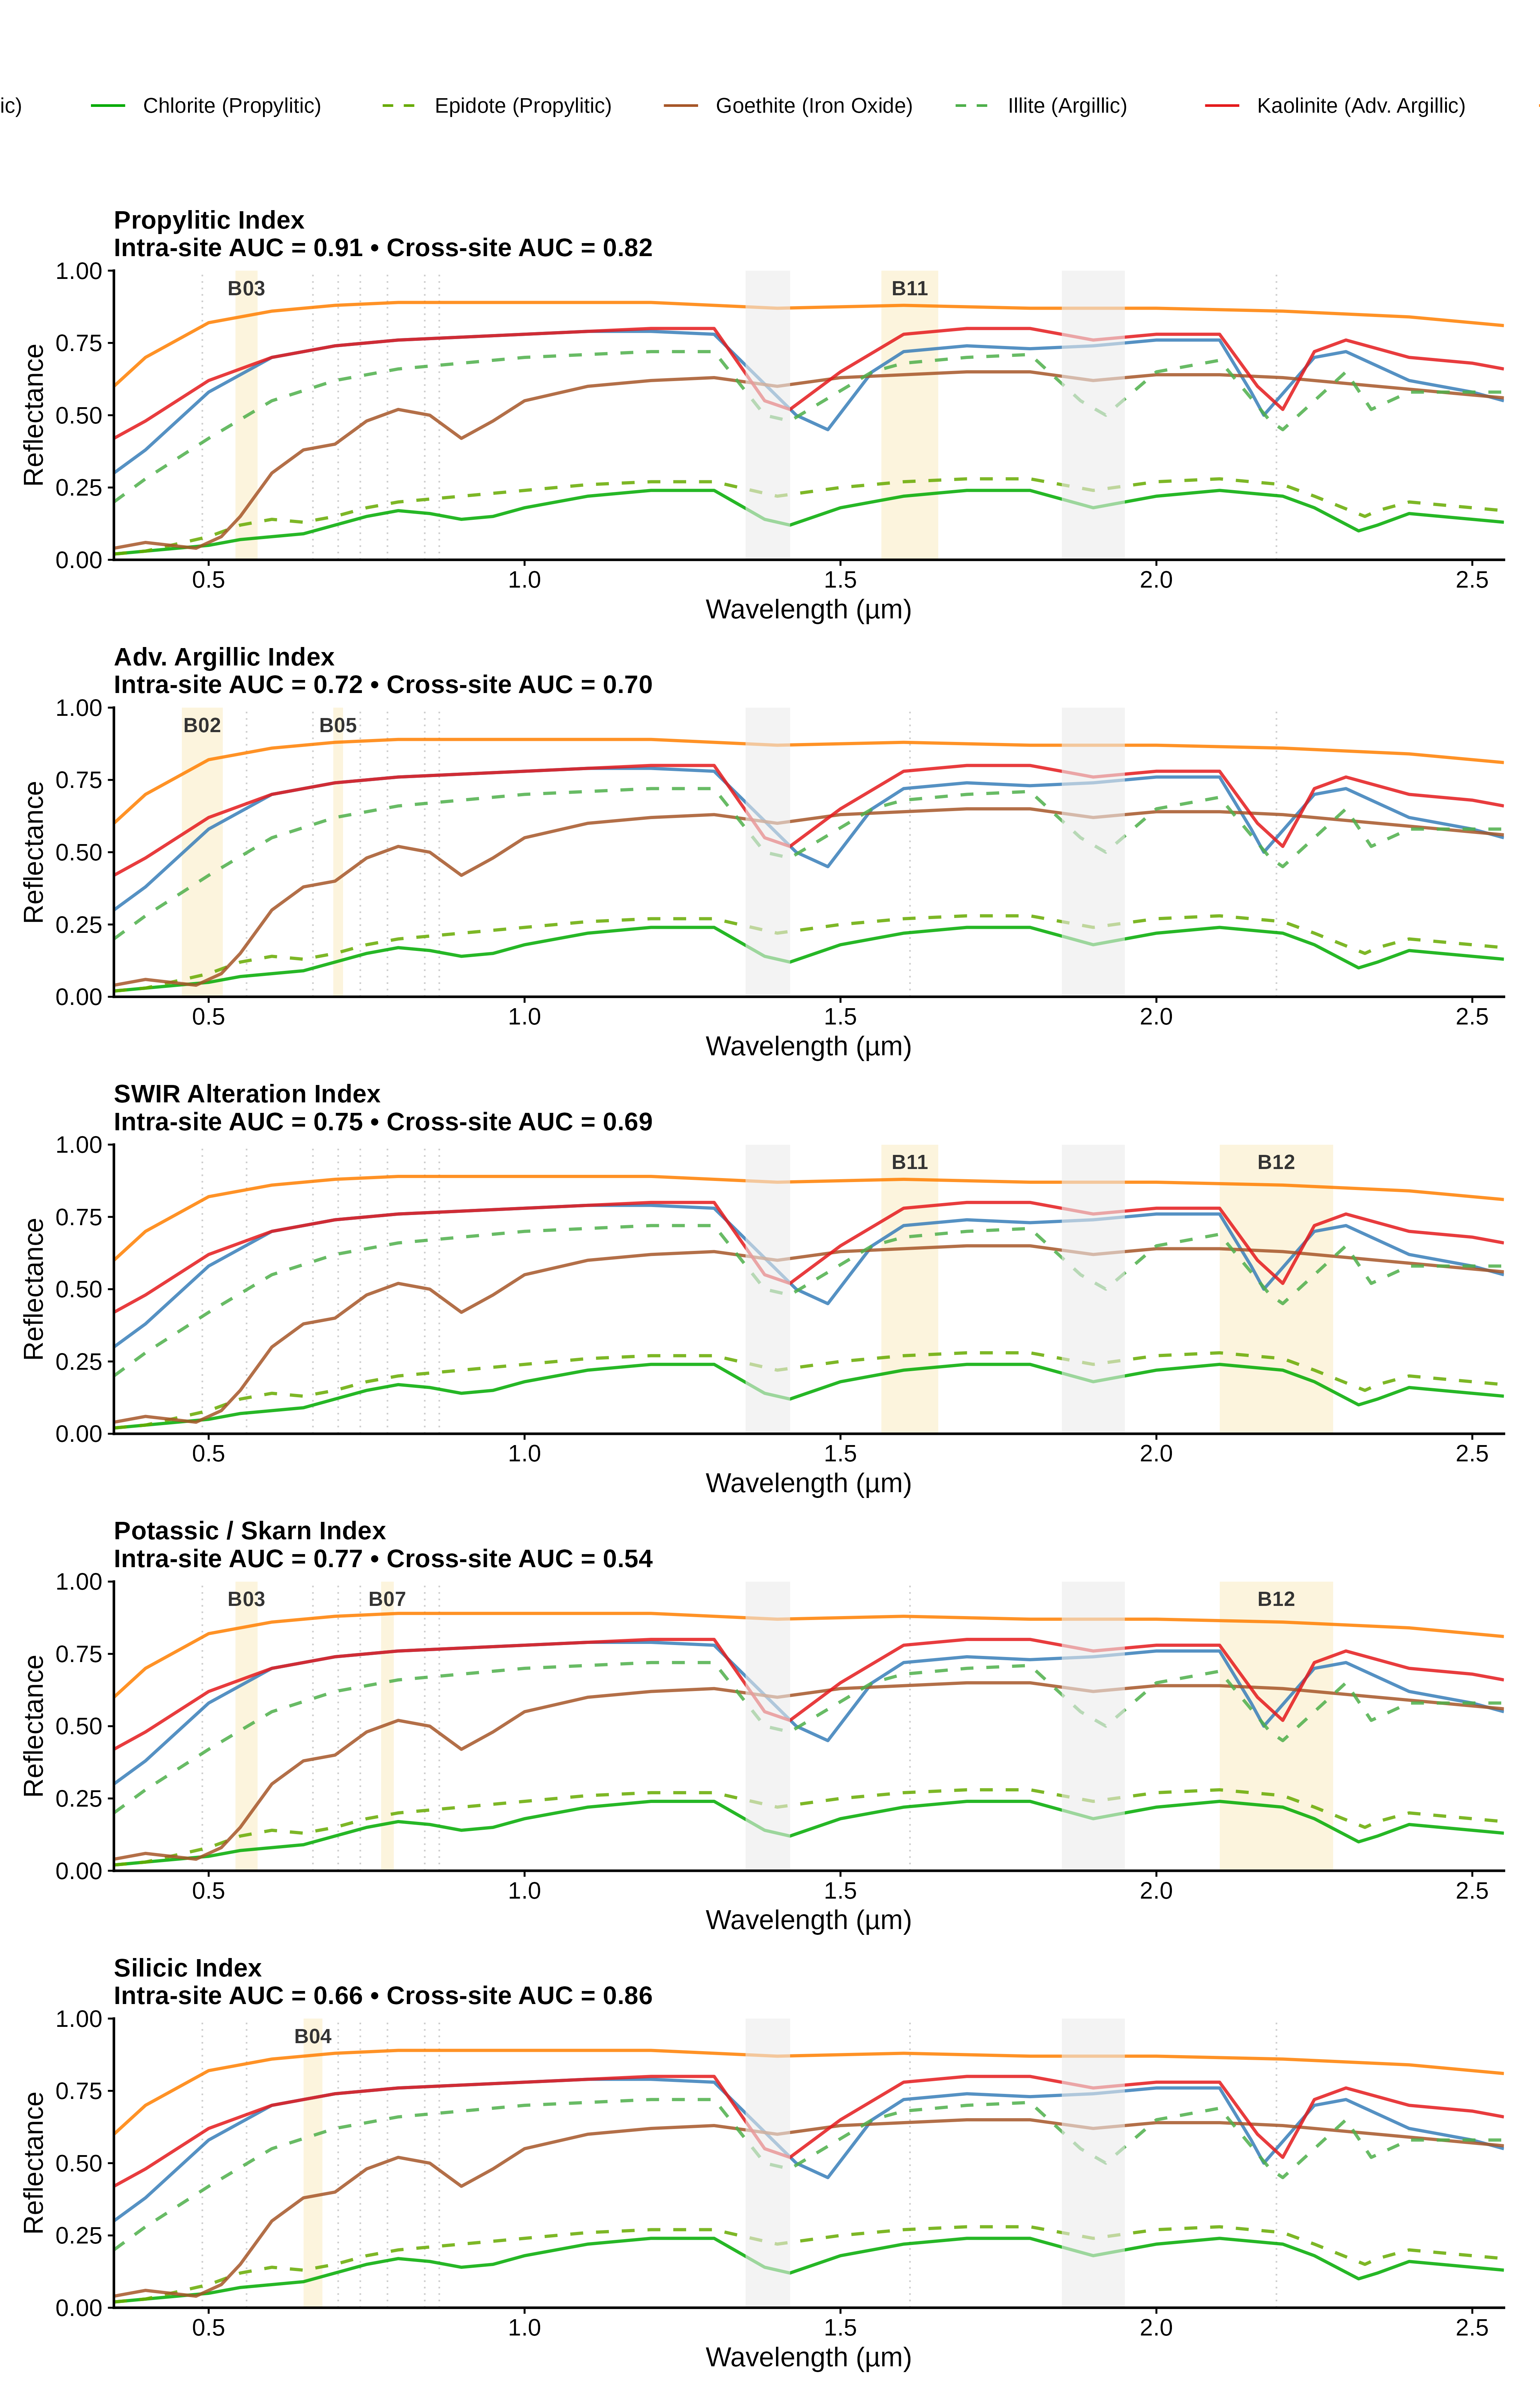
\includegraphics[width=\textwidth]{../figures/physical_interpretation.png}
\caption{Physical interpretation of SR-discovered indices. Each panel shows mineral reflectance curves (from USGS Spectral Library v7; \citealt{Kokaly2017}) overlaid with highlighted Sentinel-2 bands used by the corresponding formula. The text boxes explain the spectral mechanism that each formula plausibly exploits. Note that this overlay is interpretive, not diagnostic: the formulas are class-discriminative features whose correlation with labeled alteration classes does not imply unique spectral identification of the minerals shown (Section~\ref{sec:sr_framework}).}
\label{fig:interpretation}
\end{figure*}

% Fig. spectral_boxplots moved to Supplementary Material (Fig. S2)


%% ============================================================
\section{Discussion}
\label{sec:discussion}

\subsection{SR as Spectral Feature Engineering}

The central finding of this study is that SR-discovered indices serve a dual role: as standalone interpretable tools and as effective features for machine learning classifiers. Under the leakage-free nested protocol, the combination of SR and classical features significantly outperforms the raw bands (mean AUC 0.917 vs.\ 0.899 stratified; 0.838 vs.\ 0.822 polygon-disjoint) while using fewer features than the raw-plus-classical alternative, and the SR features alone retain 98--99\% of the raw-band performance. This is a form of automated, physics-informed feature engineering: the formulas are not arbitrary dimensionality reductions but spectral operations grounded in mineral absorption physics, and the nested design guarantees that their apparent value is not an artifact of discovery leakage.

The superiority of SR features over classical indices as RF inputs (nested mean AUC 0.889 vs.\ 0.878) further indicates that data-driven formula discovery produces more informative spectral transformations than expert-designed ratios, even after paying its discovery cost. The best performance is achieved by combining both (0.917), indicating that the two feature families are partially complementary: SR indices capture non-linear band relationships that classical ratios miss, while classical indices like NDVI and the Ferrous ratio provide spectral contrasts not targeted by the class-specific SR formulas.

\subsection{Standalone Index Performance}

As standalone spectral indices, the SR formulas offer interpretability and portability that trained models cannot. Each formula can be computed in any raster calculator (QGIS, ArcGIS, Google Earth Engine) without specialized software (Fig.~\ref{fig:alteration_maps}). The propylitic index (AUC 0.91; DeLong $p < 0.001$) and silicic index (cross-site AUC 0.86) significantly outperform classical indices for their target classes.

However, standalone SR indices underperform RF across all classes (AUC 0.62--0.91 vs.\ 0.84--0.99). This gap is expected: a single formula optimized for one class cannot match a 200-tree ensemble using all features. The practical choice between standalone indices and ensemble classification depends on the application: rapid regional screening favors standalone formulas, while detailed alteration mapping warrants the ensemble approach.

Unlike generic ratio adaptations from ASTER, the SR formulas are optimized for Sentinel-2's spectral configuration, exploiting Red Edge bands (B05, B07) that ASTER lacks.

A false positive analysis tested the six SR indices against non-altered lithologies in Region~III (fresh andesite, granitoids, sedimentary rocks, basalt, alluvium, greenschist). All indices produce weakly positive scores on most lithologies, because the spectral differences between altered and unaltered surfaces are gradational, not binary. The propylitic index, for example, yields mean scores of +0.02 to +0.05 on unaltered rocks vs.\ +0.08 to +0.15 on confirmed propylitic zones, a discrimination that is statistically significant (AUC = 0.91) but requires an appropriate threshold. In operational use, the indices should be applied with site-calibrated thresholds rather than the na\"ive sign convention. The ensemble approach (RF on SR features) inherently learns optimal thresholds and is therefore preferable for mapping applications.

\subsection{Cross-site Transferability}

The cross-site results are read through the formula-versus-method transferability distinction introduced in Section~\ref{sec:results}: formula transferability is a property of individual indices and varies with geological context, whereas method transferability (confirmed across two continents (Section~\ref{sec:cuprite_results}))is the methodological contribution of this study.

Cross-site validation from Region~III to Region~IV (a geologically independent site approximately \SI{200}{\kilo\meter} distant within the same Andean metallogenic belt)revealed heterogeneous transferability across alteration types. The silicic (AUC 0.83) and propylitic (0.82) indices transferred well, likely because both encode spectral contrasts (Green-to-SWIR in either case)rather than site-calibrated reflectance levels. The advanced argillic index maintained reasonable performance (0.70), while the argillic-phyllic index performed only marginally above chance (0.55). The iron-oxide and potassic-skarn indices could not be evaluated cross-site at all: the Region~IV ground truth distinguishes only four alteration classes (Section~\ref{sec:study_areas}) and maps neither of them, so their transferability remains untested and no claim is made about it here.

The argillic-phyllic result deserves explicit discussion. The discovered formula ($(B_{03} + 0.105)/B_{04} - 0.83$) reaches AUC = 0.65 intra-site but only 0.55 across sites, the weakest transfer of the four evaluable classes. This likely reflects the fundamental spectral similarity between argillic-phyllic and advanced argillic alteration in the VNIR--SWIR region: the diagnostic Al-OH absorption features at \SIrange{2.16}{2.20}{\micro\meter} fall within a single Sentinel-2 band (B12), preventing the discrimination that ASTER's multiple SWIR bands enable. We consider this index unreliable for operational use and recommend it only as a preliminary screening tool.

The binary detection task (altered vs.\ unaltered) achieved AUC = 0.88 with a single SR formula, approaching the RF upper bound of 0.93. The gap reflects the information advantage of using all 10 bands simultaneously, but the SR formula's simplicity and transparency may outweigh this gap for practical mapping applications.

The Cuprite validation is the primary evidence in this study for the central claim of method transferability. It extends our cross-site analysis beyond the Chilean Andes to a geologically independent province (Basin and Range, Nevada) and uses an entirely different ground truth source (USGS ASTER-derived classification rather than SERNAGEOMIN field mapping), so the replication cannot be attributed to shared spectral conditioning, shared lithology, or shared label provenance. Crucially, what was tested at Cuprite was \emph{the discovery framework}, not the specific Chilean formulas: PySR was re-run on locally sampled training data with the identical configuration, and the two Chilean findings replicated quantitatively on the locked hold-out: the local SR features retain most of the raw-band performance at a discovery cost consistent with the nested Chilean estimate (0.920 vs.\ 0.933, $\Delta = -0.014$), and the SR $+$ classical combination is again the best feature set (0.939). The replication of both patterns under such different conditions is the strongest available evidence that the framework's key property, that SR recovers compact features capturing most of the essential spectral information, and complementary to expert-designed indices, regardless of the specific geological context, generalizes across continents. By contrast, the cross-site transfer of individual Chilean formulas to Cuprite (Section~\ref{sec:cuprite_results}) yielded reduced standalone AUC, confirming our overall position that what transfers is the methodology, not necessarily any particular formula. For operational deployment at a new site, the recommended workflow is: (1) collect a modest set of labeled pixels, (2) run PySR to discover site-specific formulas, and (3) use the resulting features for classification. The computational cost is modest (minutes on a standard workstation), making this practical for any remote sensing project. Generalization to vegetated terrains remains untested and would likely require site-specific SR discovery, but the framework itself is directly applicable.

\subsection{Methodological Considerations}

The choice of complexity threshold (8 nodes) for formula selection involves a trade-off. More complex formulas from the Pareto front (complexity 10--15) achieve incrementally better loss values (Fig.~\ref{fig:pareto}), but at the cost of reduced interpretability and potential overfitting. Our selection criterion favors formulas that a domain expert can evaluate at a glance.

A sensitivity analysis of PySR hyperparameters confirms that the discovered band combinations are stable. Across the full Pareto fronts, the selected bands appear in $>$78\% of formulas (e.g., B03 and B11 appear in 11 of 14 Pareto entries for propylitic). A spot-check re-running PySR for the propylitic class with parsimony values from 0.001 to 0.03 (a 30$\times$ range) consistently recovered B03 as the primary band, and with parsimony=0.001 rediscovered the original formula ($B_{03} - 0.484 \cdot B_{11}$, vs.\ the original $B_{03} - 0.48 \cdot B_{11}$). The exact coefficients vary with parsimony, but the spectral bands and mathematical structure are robust.

The one-versus-rest strategy is natural for spectral index discovery, as each index should be interpretable as a single-purpose tool. A multi-class SR formulation would produce a single complex expression that is harder to interpret and less modular. Note that PySR minimizes mean squared error, which may be influenced by class imbalance in the OvR binary targets (e.g., propylitic has only 333 positive vs.\ 10{,}167 negative pixels in the discovery partition). The use of balanced class weights in downstream RF classifiers mitigates this for the ensemble results, but standalone SR index performance for minority classes may be suboptimal.

The two-band selection constraint (Section~\ref{sec:sr_framework}) deserves an explicit justification, because it is the one place where we override what the unconstrained search returns. Applied without it, PySR's score criterion returns $B_{04} - 0.135$ for the silicic class and $0.09/B_{05}$ for argillic-phyllic. Both are degenerate: AUC is invariant to strictly monotone transformations of a score, and tree-based classifiers split on per-feature thresholds that are likewise invariant to monotone per-feature transforms, so under our evaluation protocol the first is functionally equivalent to the raw band $B_{04}$ and the second to $-B_{05}$; their fitted constants carry no information. For those two classes the unconstrained search therefore performs band \emph{selection} rather than discovering a spectral contrast, and the resulting index inherits the confounders of the underlying band: in the silicic case, an albedo response that fires on any bright surface (Section~\ref{sec:interpretation}). The constrained selection costs $0.015$ AUC for silicic and \emph{gains} $0.028$ for argillic-phyllic on the locked hold-out, and leaves downstream performance unchanged within noise ($+0.001$ stratified, $-0.000$ polygon-disjoint under nested CV). We regard that as a favourable trade: at no measurable cost in accuracy, every reported feature is a genuine multi-band contrast rather than a relabelled band. This is the concrete form of the specificity gate we advocate in Section~\ref{sec:interpretation}: the appropriate response to a parsimony criterion that can return a scalar proxy is to constrain the selection step, not to abandon the criterion.

We additionally compared against two deep learning architectures (Table~\ref{tab:dl}): a multi-layer perceptron (MLP; 2 hidden layers, 64 units, $\sim$5{,}000 parameters) and a 1D convolutional neural network (1D-CNN; 2 convolutional layers, $\sim$8{,}600 parameters), trained for 30 epochs with early stopping (additional epochs to 100 showed no improvement). A grid search over 27 hyperparameter configurations (hidden units $\in \{32, 64, 128\}$, learning rate $\in \{10^{-2}, 10^{-3}, 10^{-4}\}$, epochs $\in \{30, 60, 100\}$) found that the best-tuned MLP (128 units, $\text{lr}=0.01$, 100 epochs) achieves mean AUC = 0.933 on SR + classical features, comparable to SVM-RBF (0.926) and exceeding RF (0.920). However, the default configurations reported in Table~\ref{tab:dl} (64 units, 30 epochs) underperform, illustrating DL's sensitivity to hyperparameter tuning for small tabular datasets. This result is consistent with the general finding that deep learning excels with high-dimensional inputs (hyperspectral, spatial context) but offers no advantage for tabular, low-dimensional spectral classification \citep{Shirmard2022}. The MLP reproduces the near-parity pattern between SR features and raw bands (0.859 vs.\ 0.856; fixed-split design, as for the other non-RF classifiers).

\begin{table}[ht]
\centering
\caption{Deep learning comparison (5-fold CV, Region~III). Neither architecture outperforms tree-based ensembles (RF mAUC = 0.920, SVM-RBF = 0.926 on the same SR + classical features).}
\label{tab:dl}
\begin{tabular}{llccc}
\toprule
Model & Features & Params & BA & mAUC \\
\midrule
MLP & 10 raw bands & 5{,}254 & 0.64 & 0.856 \\
MLP & 6 SR indices & 4{,}998 & 0.64 & 0.859 \\
MLP & 6 SR + 7 classical & 5{,}446 & 0.67 & 0.878 \\
\midrule
1D-CNN & 10 raw bands & 8{,}614 & 0.52 & 0.791 \\
1D-CNN & 6 SR indices & 8{,}614 & 0.58 & 0.830 \\
1D-CNN & 6 SR + 7 classical & 8{,}614 & 0.54 & 0.792 \\
\bottomrule
\end{tabular}
\end{table}

The temporal stability of the discovered indices was not evaluated. Our analysis used a single dry-season composite (January--March 2024); seasonal variations in atmospheric conditions, soil moisture, and residual vegetation phenology could affect index values. We recommend validation across multiple years before operational deployment.

\subsection{Limitations and scope}
\label{sec:limitations}

For clarity, and to avoid over-claiming, we summarize here the main limitations that constrain the scope of the present results. The individual points are discussed in more detail in the preceding subsections and in Methods.

\begin{enumerate}
  \item \textbf{Discovery cost and spatial autocorrelation are both quantified; absolute pixel-level AUCs remain upper bounds.} Two forms of optimism affect training-site results, and this study measures both. First, label-dependent formula discovery outside the evaluation loop inflates downstream results: the nested protocol (discovery re-run inside each training fold) shows a genuine discovery cost of 0.011 (stratified) to 0.020 (polygon-disjoint) AUC that the fixed-split design understates (Table~\ref{tab:ensemble} vs.\ Table~\ref{tab:spatial_robust}). Consequently, we do not claim statistical equivalence between SR features and raw bands at $\varepsilon = 0.01$; the data support equivalence only at $\varepsilon = 0.02$--$0.03$, and we report the SR-alone result as 98--99\% retention rather than losslessness. Second, pixel-level cross-validation inflates absolute AUC through spatial autocorrelation of the mapped polygons: under polygon-disjoint and spatial block schemes, absolute mean AUC falls by 0.08--0.21, reaching 0.822 (polygon-disjoint) and 0.707 (\SI{5}{\kilo\meter} blocks) for RF(raw). The \emph{relative} findings that anchor this paper hold in every scheme, nested included: SR features outperform classical indices, and SR $+$ classical significantly outperforms the raw bands. We treat pixel-level intra-site AUCs as upper bounds and use the nested polygon-disjoint results as the defensible intra-site estimates, with Cuprite (Section~\ref{sec:cuprite_results}) as the primary out-of-site evidence.
  \item \textbf{Formula transferability varies by class, and is weakest for compositionally heterogeneous classes.} Cross-site AUC at Region~IV ranges from 0.57 (argillic-phyllic) and 0.54 (potassic-skarn) to 0.86 (silicic) and 0.82 (propylitic). This is expected for formulas with empirically fitted constants and spectrally broad target classes, and reinforces our central claim: what transfers robustly is the discovery framework, not any individual formula (Section~\ref{sec:discussion}).
  \item \textbf{Sentinel-2's two SWIR bands impose a hard upper bound on mineralogical specificity.} Narrow absorption features that diagnose specific alteration mineralogies (kaolinite doublet at \SI{2.17}{\micro\meter}, alunite at \SI{2.20}{\micro\meter}, chlorite/epidote Mg-OH at \SI{2.25}{\micro\meter}--\SI{2.35}{\micro\meter})fall inside broad Sentinel-2 bands and cannot be resolved as distinct features (Section~\ref{sec:interpretation}). SR partially compensates by exploiting VNIR and Red Edge bands that ASTER-based indices ignore, but cannot overcome this structural limitation. Hyperspectral data would be required for mineralogically sharper indices.
  \item \textbf{Ground-truth quality differs between sites and propagates to absolute AUC values.} The Atlas Metal\'ifero (Region~III/IV) provides regional-scale ($\sim$1:100{,}000) field-mapped polygons; positional accuracy is on the order of tens of meters and class boundaries reflect surface expression rather than subsurface zonation, introducing label noise that may suppress measured AUC. The Cuprite reference is itself a remote sensing product (USGS automated ASTER classification, \citealp{Rockwell2017}), well-validated against field and laboratory spectroscopy \citep{Swayze2014} but subject to its own sensor-specific biases; the high AUC values at Cuprite (0.94--0.97) may partly reflect ASTER--Sentinel-2 spectral consistency rather than purely mineralogical accuracy. In addition, the USGS ``argillic'' (kaolinite/halloysite) and ``phyllic'' (muscovite/sericite) classes do not map exactly onto the Chilean classification \citep{Sillitoe2010}. These class-boundary ambiguities affect per-class transfer comparisons but not the within-site feature-engineering equivalence that anchors our central claim.
  \item \textbf{Class imbalance affects standalone minority-class performance.} PySR minimizes MSE on the OvR binary target, and minority classes (e.g., propylitic: 333 positives vs.\ 10{,}167 negatives) yield formulas whose standalone AUC may be suboptimal relative to a balanced reformulation. Downstream RF classifiers use balanced class weights and mitigate this for the ensemble results.
  \item \textbf{We do not claim universality of the specific formulas reported here.} The discovered expressions are optimized for the arid, high-altitude, minimally vegetated context of the Chilean Andes training site. They should not be applied without validation to settings with significant vegetation cover, different atmospheric conditions, or non-volcanic lithologies. Consistent with our scope, the transferable product of this study is the discovery framework: a practitioner working in a tropical porphyry system, a geothermal field outside the Andes, or a non-geological remote sensing domain would re-run SR on local labeled data and likely discover different formulas reflecting the local spectral context.
  \item \textbf{SR and PCA address different requirements within the accuracy--interpretability trade-off.} As shown in Table~\ref{tab:spatial_robust}, RF(PCA 6 components) achieves a higher absolute AUC than the nested RF(6 SR features) by roughly $0.05$--$0.06$, and even exceeds RF on the ten raw bands; PCA therefore yields the strongest 6-feature linear representation of Sentinel-2 in this task. SR(6) retains 98--99\% of the raw-band accuracy, with the additional properties of closed-form expressibility, sensor-agnostic portability, and direct mineral-spectroscopic interpretability that PCA's fitted transformation matrix does not provide. The two representations therefore answer different questions and are complementary rather than substitutable: PCA is preferable when the feature set is internal to a downstream classifier, whereas SR is preferable when the features themselves must be auditable, deployable as algebra in any raster calculator, and inspectable by a domain expert.
\end{enumerate}

These limitations define the scope of our claims but do not weaken the central findings. The complementarity of SR and classical features (significant under leakage-free nested validation), the 98--99\% retention achieved by the SR features alone, the replication of both patterns at Cuprite under entirely different geological and ground-truth conditions, and the interpretability of the discovered expressions are robust to all of the points above.

\subsection{Cross-domain proof-of-concept: land cover classification}
\label{sec:crossdomain}

The method transferability tested at Cuprite (Section~\ref{sec:cuprite_results}) concerns a different continent and geological province but still the same application domain (hydrothermal alteration mapping). As a secondary test (not to shift the focus away from geology but to probe whether the feature engineering pattern is intrinsically tied to alteration mapping at all)we applied the identical SR framework to a non-geological problem: land cover classification using ESA WorldCover 2021 labels and Sentinel-2 imagery from central Germany (five classes: Forest, Grassland, Cropland, Built-up, Water; 6{,}612 pixels). The key pattern replicates: RF trained on SR + classical features (mean AUC = 0.926) exceeds RF on 10 raw bands (0.920), while SR indices alone achieve 0.902. The land cover SR formulas are dominated by the NIR band (B08 in 4 of 5 formulas), contrasting with the visible--SWIR emphasis of the alteration indices, though SWIR bands also contribute to land cover discrimination, confirming that SR adapts to the spectral characteristics of the target domain rather than reproducing any fixed preference. Full results are reported in Supplementary Table~S5. The main scientific contribution of this paper remains geological remote sensing; this cross-domain result is reported as supporting evidence for framework generality.


%% ============================================================
\section{Conclusions}
\label{sec:conclusions}

We demonstrated that symbolic regression is a general-purpose, transferable framework for automated spectral feature engineering, evaluated under a leakage-free nested protocol in which formula discovery is re-run inside every training fold. The central claim of this work concerns \emph{method transferability} (that the SR discovery process consistently yields compact and effective features when re-applied under new geological conditions)rather than the universal optimality of any particular formula. The framework requires only labeled pixels and a sensor's band configuration, and can be re-applied at any new site to discover locally optimal indices, making it a practical tool for any remote sensing classification problem. Using hydrothermal alteration mapping from Sentinel-2 as a challenging test case (six spectrally similar classes, three sites across two continents), we discovered six class-specific indices using 1--3 spectral bands each. Key findings include:

\begin{enumerate}
  \item SR-derived and classical indices are complementary: a Random Forest on six SR features plus seven classical indices significantly outperforms the same classifier on all ten raw Sentinel-2 bands under stratified nested CV (mean AUC 0.917 vs.\ 0.899, $p = 0.002$) and under polygon-disjoint spatial nested CV (0.838 vs.\ 0.822, $p = 0.008$), with fewer features than the raw-plus-classical alternative. The pattern holds across four classifiers and two deep learning architectures.
  \item The six SR features alone retain 98--99\% of the raw-band discriminative performance (nested mean AUC 0.889 vs.\ 0.899; 0.802 vs.\ 0.822 polygon-disjoint). The nested protocol quantifies an honest discovery cost of 0.01--0.02 AUC that fixed-split designs understate, and shows that discovery is stable: the strongest formulas are rediscovered nearly verbatim across independent training partitions.
  \item Both findings replicate at Cuprite, Nevada (USA) (a geologically independent benchmark on a different continent)using formulas discovered locally by the identical configuration (SR $+$ classical 0.939 vs.\ raw 0.933; SR alone 0.920, $\Delta = -0.014$), confirming that the \emph{methodology} generalizes across geological provinces, rather than only the specific formulas.
  \item As standalone indices, the propylitic formula ($B_{03} - 0.48 \cdot B_{11}$; AUC = 0.91 on a locked hold-out; DeLong $p < 0.001$) significantly outperforms classical spectral indices for its target class. Standalone transferability varies by class, as expected for formulas with empirically fitted constants.
  \item The discovered formulas exploit spectral features consistent with mineral absorption theory, bridging data-driven optimization and physics-informed interpretation.
  \item A cross-domain proof-of-concept on land cover classification (five classes, central Germany) replicates the key pattern: SR + classical features exceed raw bands (mean AUC 0.926 vs.\ 0.920), supporting the generalization of the framework to non-geological multispectral classification problems.
\end{enumerate}

Three concluding points frame the scope of this work.

\emph{What this paper contributes.} The main outcome is methodological: symbolic regression provides a practical route to discover compact, interpretable, and site-redeployable spectral features from labeled multispectral data, and nested cross-validation provides the correct protocol for evaluating any such label-dependent feature discovery. The significant complementarity of SR and classical features under that protocol, the 98--99\% retention achieved by the SR features alone, and the replication of both at Cuprite across an independent geological province and an independent ground-truth source are, together, the strongest empirical support for this claim.

\emph{What this paper does not claim.} We do not conclude that the specific formulas reported here are universally optimal, nor that they supersede the classical ASTER-era indices in every geological setting. Standalone transferability varies by class, and the discovered expressions reflect the spectral characteristics of the arid Andean training context. The transferable product of this study is the discovery strategy, not a fixed library of indices.

\emph{Why this matters.} The methodology positions symbolic regression as a general-purpose bridge between domain-driven and data-driven approaches in multispectral remote sensing, particularly relevant where scientific interpretability and GIS portability matter as much as predictive accuracy. The framework is broadly applicable across classification domains (vegetation, soil, water quality, urban materials) and across multispectral sensors where labeled pixels are available; the recommended workflow at a new site or domain is straightforward: collect labeled pixels, run SR to discover locally appropriate formulas, and use the resulting features for classification.


%% ============================================================
\section*{Data Availability}

Sentinel-2 L2A imagery is freely available from the Copernicus Open Access Hub and Google Earth Engine. Ground truth data from the Atlas Metal\'ifero de la III Regi\'on are available from SERNAGEOMIN (Chile). Code for the symbolic regression pipeline (including the nested cross-validation experiments), the discovered formulas, and the extracted per-pixel training tables for all three sites are available at \url{https://github.com/franciscoparrao/spectral-indices-discovery}; an archival snapshot with DOI will be deposited on Zenodo upon acceptance. Because GEE temporal composites are not guaranteed to be bit-reproducible over time, the deposited pixel tables are the reference data for reproducing all reported numbers.

\section*{CRediT Author Statement}

\textbf{Francisco Parra~O.}: Conceptualization, Methodology, Software, Validation, Formal Analysis, Investigation, Data Curation, Writing -- Original Draft, Writing -- Review \& Editing, Visualization.
\textbf{Gonzalo R\'ios}: Validation, Writing -- Review \& Editing.
\textbf{Mauricio Latorre}: Validation, Writing -- Review \& Editing.

\section*{Declaration of Competing Interest}

The author declares no competing interests.

\section*{Funding}

This research did not receive any specific grant from funding agencies in the public, commercial, or not-for-profit sectors.

\section*{Declaration of Generative AI and AI-assisted Technologies in the Manuscript Preparation Process}

During the preparation of this work the author used Claude (Anthropic) in order to assist with code development for the analysis pipeline, figure generation scripts, and manuscript drafting. After using this tool, the author reviewed and edited the content as needed and takes full responsibility for the content of the published article.

\section*{Acknowledgements}

The authors acknowledge SERNAGEOMIN for making the Atlas Metal\'ifero de la III Regi\'on publicly available. Sentinel-2 data were accessed through Google Earth Engine \citep{Gorelick2017}. Symbolic regression was performed using the PySR library \citep{Cranmer2023}. USGS alteration data for Cuprite were accessed via the WMS service at \texttt{mrdata.usgs.gov} \citep{Rockwell2017}. Mineral spectral reference curves are from the USGS Spectral Library v7 \citep{Kokaly2017}.

F.P.\ acknowledges funding support from the Postdoctorate 2026 Project, Code 062619MC\_POSTDOC, Vicerrector\'\i a de Investigaci\'on, Innovaci\'on y Creaci\'on, Universidad de Santiago de Chile.

M.L.\ acknowledges support from ANID Anillo Regular ACT210004; Center for Mathematical Modeling, Apoyo a Centros de Excelencia ACE210010; ANID Millennium Science Initiative Program ICN2021\_044; Fondo Basal FB210005; ANID FONDECYT 1230194; and the Fondo Interdisciplinario y Proyecto N\'ucleo UOH.


%% ============================================================
%% REFERENCES
%% ============================================================
\bibliographystyle{elsarticle-harv}
\bibliography{references}

\end{document}
